% \documentclass[a4paper,12pt,twoside]{scrreprt}
\documentclass[a4paper,12pt,tikz]{scrreprt}


% Für deutsche Überschriften, usw. dieses Paket aktivieren
% \usepackage[ngerman]{babel}

%% REQUIRED PACKAGES
\usepackage{amsfonts,amsmath,amssymb} % math stuff
\usepackage{booktabs} % better layout for tables
\usepackage{color} % enable use of colors
\usepackage{fancyhdr} % definition of own headers/footers
\usepackage{graphicx,wrapfig} % for including pictures
\usepackage{units} % for giving quantities the right surrounding
\usepackage{xspace} % correct spacing behind DuMuX command
\usepackage[version=4]{mhchem} % better layout for chemical notation

%% CSV FILE PACKAGE
\usepackage{booktabs} % For \toprule, \midrule and \bottomrule
\usepackage{siunitx} % Formats the units and values
\usepackage{pgfplotstable} % Generates table from .csv
\usepackage[np, autolanguage]{numprint}
\usepackage{siunitx}
\sisetup{output-exponent-marker=\ensuremath{\mathrm{e}}}
\setlength{\tabcolsep}{12pt}
\renewcommand{\arraystretch}{1.3}

% Setup siunitx:
\sisetup{
  round-mode          = places, % Rounds numbers
  round-precision     = 2, % to 2 places
}

\usepackage{pgfplots}
\pgfplotsset{compat=newest} % Allows to place the legend below plot
\usepgfplotslibrary{units} % Allows to enter the units nicely

\usepackage{csvsimple,longtable,booktabs}
\setlength{\topmargin}{-10.4mm}
\setlength{\headheight}{0.0mm}
\setlength{\headsep}{10.0mm}
\setlength{\textwidth}{160mm}
\setlength{\textheight}{242mm}
\setlength{\oddsidemargin}{0mm}
\setlength{\evensidemargin}{0mm}
\setlength{\marginparwidth}{0mm}
\setlength{\marginparsep}{0mm}

%% PACKAGE FOR FLOWCHART
\usepackage{tikz}
\usepackage{flowchart}
\usetikzlibrary{arrows}
\usetikzlibrary{shapes.geometric, arrows}
\tikzstyle{startstop} = [rectangle, rounded corners, minimum width=3cm, minimum height=1cm,text centered, draw=black]

\tikzstyle{connector} = [circle, radius=3cm, text centered, draw=black]

\tikzstyle{io} = [trapezium, trapezium left angle=70, trapezium right angle=110, minimum width=5cm, minimum height=1cm, text centered, text width= 5cm, draw=black]

\tikzstyle{process} = [rectangle, rounded corners, minimum width=3cm, minimum height=1cm, text centered, text width= 7cm, draw=black]

\tikzstyle{decision} = [diamond, minimum width=3cm, minimum height=1cm, text centered, text width= 3cm, draw=black]

\tikzstyle{predefinedprocess} = [draw, predproc, minimum width=3cm, minimum height=1cm, text centered, text width= 7cm, draw=black]

\tikzstyle{arrow} = [thick,->,>=stealth]

%%
\tikzstyle{block} = [rectangle, draw, 
    text width=17em, text centered, rounded corners, minimum height=3em]
    
\tikzstyle{description} = [rectangle, draw, 
    text width=15em, text centered, rounded corners, minimum height=3em]
    
\tikzstyle{line} = [draw, -latex']
\tikzstyle{cloud} = [draw, predproc, text width=15em, text centered, minimum height=3em]
\tikzstyle{dec} = [diamond, text width=5em, text centered, minimum height=4em]

%% Package for sub-plots
\usepackage{caption}
\usepackage{subcaption}

%% OPTIONAL PACKAGES
\usepackage[labelfont=bf]{caption}
\captionsetup{labelfont=bf}
\usepackage{chngcntr}
\counterwithout{figure}{chapter}
\usepackage{array}
\usepackage{makecell}

\renewcommand\theadalign{bc}
\renewcommand\theadfont{\bfseries}
\renewcommand\theadgape{\Gape[4pt]}
\renewcommand\cellgape{\Gape[4pt]}

\usepackage[export]{adjustbox}
\usepackage[titles]{tocloft}
\renewcommand{\cftdot}{}
\usepackage{chemformula}%loaded by chemmacros
\usepackage{array} % needed for the new column type
\usepackage{lipsum} % dummy text with \lipsum[1]
\usepackage{subcaption} % multiple figures in one row
\usepackage{rotating} % rotating of figures
\usepackage{todonotes} % for colorful todo notes
% \usepackage[nottoc]{tocbibind} % for list of figures and tables
\usepackage{dirtytalk} % package for quote
% \usepackage[style=authoryear]{biblatex}
% \usepackage[square]{natbib}
\usepackage[numbers]{natbib}
% \bibliographystyle{abbrv}
% \setcitestyle{authoryear,open={(},close={)}}
\usepackage[colorlinks=true,linkcolor=black,bookmarks=true,bookmarksopen=true,bookmarksopenlevel=2]{hyperref} % enable links
\hypersetup{
%  pdfpagemode=None,
  citecolor=cyan,
  pdfpagemode=UseOutlines,
  pdfstartview=Fit,
  pdftitle={},
  pdfsubject={},
  pdfauthor={},
  pdfkeywords={},
  pdfcreator={pdflatex}
}
\usepackage{cleveref}
\usepackage{physics}
\newcommand{\comment}[1]{} % FOR COMMENTING
%% PAGE SETUP
\textheight 22.5cm
\textwidth 15.5cm
\oddsidemargin 0.5cm
\evensidemargin 0.5cm
\parindent 0cm
\topmargin 0cm

%% NUMERATION OF ELEMENTS
\setcounter{secnumdepth}{5} % depth of numeration, including \subparagraph
\renewcommand{\theequation}{\thechapter.\arabic{equation}} % numeration for equations
\numberwithin{equation}{chapter}
\renewcommand{\thefigure}{\thechapter.\arabic{figure}} % numeration for figures
\numberwithin{figure}{chapter}
\renewcommand{\thetable}{\thechapter.\arabic{table}} % numeration for tables
\numberwithin{table}{chapter}

%% TEXT APPEARANCE
\renewcommand{\labelitemi}{$-$} % char for itemize environments
\renewcommand{\baselinestretch}{1.05} % line spacing
\newcommand{\code}{\texttt}

%% USER DEFINED SETUP
\newcolumntype{V}[1]{>{\raggedright\hspace{0pt}}p{#1}} % columntype with word wrap
\newcommand{\Pics}{./PICTURES} % path to figures
\newcommand{\DuMuX}{DuMu$^\textrm{x}$\xspace}
\newcommand{\MATLAB}{\textsc{M\footnotesize{ATLAB}}\xspace}

\begin{document}

\setcounter{page}{-1}  % exclude title page from numbering
% \pdfbookmark[0]{Title Page}{Title Page}
%% PAGE SETUP
\thispagestyle{empty} % no page number, header or footer

\vspace*{-2truecm}

\newlength{\HeadWidth}
\setlength{\HeadWidth}{\textwidth}

\newlength{\LogoWidthL}
\settowidth{\LogoWidthL}{
\includegraphics[height=20mm]{./PICTURES/Logo_UniS-zentriert}}
\addtolength{\HeadWidth}{-\LogoWidthL}
\addtolength{\HeadWidth}{-3mm} % for correction

\newlength{\LogoWidthR}
\settowidth{\LogoWidthR}{
\includegraphics[height=23mm]{./PICTURES/Logo_LH2_sw}}
\addtolength{\HeadWidth}{-\LogoWidthR}
\addtolength{\HeadWidth}{-3mm} % for correction

\newlength{\BoxBreite}
\setlength{\BoxBreite}{\textwidth}

\vspace*{-1.5cm}
{
  \parbox[b]{\BoxBreite}
  {                               
    
\includegraphics[height=20mm]{\Pics/Logo_UniS-zentriert}
    \parbox[b][22mm][c]{\HeadWidth}
    {                                       
      \fontsize{10}{11pt}\selectfont \sffamily        
      \begin{center}          
        Universit\"at Stuttgart  -  Institut f\"ur Wasser- und Umweltsystemmodellierung\\    
        {\bfseries 
          Lehrstuhl f\"ur Hydromechanik und Hydrosystemmodellierung}\\
        Prof.~Dr.-Ing.~Rainer Helmig    
      \end{center} 
      }
    
\includegraphics[height=23mm]{\Pics/Logo_LH2_sw} \\ [-3mm] 
    }
  }       
\vspace{3cm}

%% TEXT PART
\begin{center}
   {\large Master's Thesis}\\[0.5cm]
  {\bfseries {\LARGE Modeling calcite dissolution due to
density-induced fingering of CO\textsubscript{2}-enriched water\\[0.3cm]}}
\end{center}

\vspace{5cm}

\begin{center}
  {\normalsize Submitted by:}\\[0.1cm]
  {\large Animesh Nepal}\\[0.1cm]
\end{center}

\vspace{3cm}

\begin{center}
  {\large Stuttgart, November 24, 2020}
\end{center}

\vspace{0.5cm}

\begin{center}
  {\large 
  \begin{tabular}{ll}
  \textbf{Examiners:}& apl. Prof. Dr.-Ing. Holger Class\\ & apl. Prof. Dr. rer. nat. Bernd Flemisch\\
  \textbf{Supervisors:}& Dr.-Ing. Kilian Weishaupt\\ & Dr.-Ing. Johannes Hommel
  \end{tabular}
  }\\[0.1cm]
\end{center}

\endinput
\cleardoublepage % blank page for twoside print

\pagenumbering{Roman} % first pages have Roman numbering
\setcounter{page}{1}  % exclude title page from numbering


%% SETUP OF HEADER AND FOOTER
\pagestyle{fancy}
\renewcommand{\chaptermark}[1]{\markboth{#1}{}}
\renewcommand{\sectionmark}[1]{\markright{\thesection\ #1}}
\fancyfoot{}
\fancyhead{}
\fancyhead[LE,RO]{\small\bfseries \thepage}
\fancyhead[LO]{\small\bfseries \rightmark}
\fancyhead[RE]{\small\bfseries \leftmark}
\renewcommand{\headrulewidth}{0.5pt} % thin line in headers


%% REQUIRED PAGES
\newpage
\thispagestyle{empty}

\vspace*{\fill}
%use the English or the German version according to the language used in your thesis.

I hereby certify that I have prepared this thesis independently, and that only
those sources, aids, and advisors that are duly noted herein have been used
and/or consulted.

I further agree that this thesis is made accessible for scientific purposes by the
library of the Institute for Modelling Hydraulic and Environmental Systems of
the University of Stuttgart (Publication according to {\S}6 Abs. 1 UrhG).
I agree that contents may be cited according to {\S}52 UrhG.\\[1cm]
Stuttgart, November 24, 2020\\[2cm]
Animesh Nepal \\

\endinput % UNCOMMENT
\cleardoublepage % blank page for twoside print
\chapter*{Acknowledgements}
\thispagestyle{empty}
I would like to express my deep and sincere gratitude to Holger Class for giving me the opportunity 
to conduct the thesis at the department LH\textsuperscript{2} and guiding me throughout the thesis. 
His insights into the subject were fundamental in making key decisions during the thesis. 
I also thank him for his trust in me on this task and for reminding me the big-picture, which 
served as a motivation for me to conduct this study, and at the same time helping me understand 
important details. \\

I would also like to thank Johannes Hommel who has been invaluable for this thesis to materialize. 
I was able to infer help from his dissertation to calculate and model the rate of dissolution of calcite. 
I would also like to thank Kilian Weishaupt for his help and time during online meetings in setting 
Fluid-system in DuMu\textsuperscript{x}, and for the model he developed for density-driven flow, 
which was my reference while implementing the model in DuMu\textsuperscript{x}. His help, together 
with Johannes, in understanding and rectifying the compiler errors while implementing the model in 
DuMu\textsuperscript{x} was crucial in finishing the thesis in the stipulated time.\\

I would like to thank Martin Schneider helping me setting up DuMu\textsuperscript{x} in VS Code 
and in running a debugger, which proved very handy in identifying and rectifying the errors in the code. \\
I would also like to thank Bernd Flemisch for his help in setting a git repository, which was essential 
to collaborate the work with different members.
\endinput % UNCOMMENT
\cleardoublepage % blank page for twoside print


%% TABLE OF CONTENTS AND LISTS
\tableofcontents
\newpage
\pagenumbering{Roman}
\addcontentsline{toc}{chapter}{List of Figures}
\listoffigures \newpage
\addcontentsline{toc}{chapter}{List of Tables}
\listoftables \newpage
\addcontentsline{toc}{chapter}{nomenclature}
\chapter*{Nomenclature}
% \pdfbookmark[1]{Abstract}{Abstract}
\thispagestyle{empty}

The following tables show the symbols and their definitions used in this thesis.

\begin{table}[h!]
    \small\addtolength{\tabcolsep}{0pt}
    \label{tab:notation}
    \begin{tabular}{lll} % <-- Changed to S here.
    \hline
      \textbf{Symbol} & \textbf{Definition} & \textbf{Dimension}\\
      \hline
      \textbf{D} & Binary diffusion constant & [\ce{m^2}/s]\\
      \ce{A_{cw}} & surface area of calcite & [\ce{m^2}/\ce{m^3}] \\
      $\gamma^\kappa$ & activity coefficient of component $\kappa$ & [-]\\
      $\mu$ & dynamic fluid viscosity & [kg/ms] \\
      $\nu$ & kinematic fluid viscosity & [\ce{m^2}/s] \\
      $\rho$ & fluid density & [kg/\ce{m^3}] \\
      $\rho_0$ & initial density of the fluid & [kg/\ce{m^3}] \\
      \textbf{v} & velocity vector & [m/s] \\
      p & pressure & [kg/m\ce{s^2}] \\
      g & gravity & [m/\ce{s^2}] \\
      \textbf{g} & gravity vector & [\ce{m^2/s}] \\
      $\Omega$ & calcite saturation index & [-] \\
      \hline
    \end{tabular}
%   \end{center}
\end{table}

\begin{table}[h!]
    \small\addtolength{\tabcolsep}{-4pt}
    \label{tab:notation}
    \begin{tabular}{ll} % <-- Changed to S here.
      \hline
      \thead{Superscripts/Acronyms} &  \thead{Definition} \\
      \hline
      $\kappa$ & component \\
      Ca, \ce{Ca^{2+}} & calcium  \\
      \ce{CO2} & carbon dioxide  \\
      \ce{CaCO3} & calcium carbonate/ calcite  \\
      \ce{H2O} & water  \\
      \ce{CO3^{2-}} & carbonate  \\
      \ce{HCO3^-} & bicarbonate  \\
      \ce{H^+} & hydrogen ion  \\
      \ce{OH^-} & hydroxide ion  \\
      \ce{H2CO3} & carbonic acid  \\
      w & water  \\
      TIC & total inorganic carbon \\
      NS & Navier-Stokes \\
\end{tabular}
\end{table}


\begin{table}[h!]
    \small\addtolength{\tabcolsep}{-4pt}
    \label{tab:notation}
    \begin{tabular}{lll} % <-- Changed to S here.
      \hline
      \thead{Chemical notation} & \thead{Definition} & \thead{Dimension} \\
      \hline
      $\ce{m^{TIC}}$ & molality of TIC & [\ce{mol_{TIC}}/\ce{kg_{\ce{H2O}}}]\\
      $\ce{m^{Ca^{2+}}}$ & molality of calcium & [\ce{mol_{\ce{Ca^{2+}}}}/\ce{kg_{\ce{H2O}}}] \\
      $\ce{m^{CO_3^{2-}}}$ & molality of carbonate & [\ce{mol_{\ce{CO_3^{2-}}}}/\ce{kg_{\ce{H2O}}}] \\
      $\ce{\ce{m^{HCO_3^{-}}}}$ & molality of bicarbonate & [\ce{mol_{\ce{HCO_3^{-}}}}/\ce{kg_{\ce{H2O}}}] \\
      $\ce{m^{H^+}}$ & molality of hydrogen & [\ce{mol_{\ce{H^+}}}/\ce{kg_{\ce{H2O}}}] \\
      
      \ce{r_{diss}} & rate of calcite dissolution & [mol/\ce{m^3}s] \\
      \ce{k_{diss,1}} & dissolution constant &  [\ce{mol_{\ce{Ca^{2+}}}/\ce{m^2s}}]/[\ce{mol_{H}}/\ce{kg_{\ce{H2O}}}] \\
      \ce{k_{diss,2}} & dissolution constant & [\ce{mol_{\ce{Ca^{2+}}}}/\ce{m^2}s]\\
      \ce{K_{sp}} & solubility product of calcite & [\ce{mol^2/kg^2_{\ce{H2O}}}] \\
      \ce{q^{TIC}} & source term for total inorganic carbon & [mol/\ce{m^3}s] \\
      \ce{q^{Ca}} & source term for calcium & [mol/\ce{m^3}s] \\
    \end{tabular}
%   \end{center}
\end{table}





\endinput \newpage
\addcontentsline{toc}{chapter}{Abstract}
\chapter*{Abstract}
% \pdfbookmark[1]{Abstract}{Abstract}
\thispagestyle{empty}
Density-induced fingering due to dissolution of \ce{CO2} in water is considered a mechanism for 
speleogenesis. \citet{Scherzer2017} stated this process as \say{Nerochytic Speleogenesis} (NERO). 
Despite having similar effects to density-driven fingering of \ce{CO2} in geological sequestration 
of greenhouse gases, it is so far not discussed as a mechanism for speleogenesis. Understanding the 
process could help in understanding karst formation, also known as karstification.\\

We developed a model in \DuMuX, also validated with \MATLAB, that considered the dissolution of calcium-carbonate 
as a source/sink term in the Navier-Stokes model. We found the concentration of \ce{CO2} at the top of 
the cave water table that leads to a concentration gradient between the region above and below the epiphreatic karst water table, 
and the flow-velocity to influence the rate of calcite dissolution. We ran simulations for different 
scenarios and compared the results to see the effects on the rate of calcite dissolution. The numerical comparison 
between \DuMuX and \MATLAB showed consistency in predicting the rate of calcite dissolution. \\

Modeling a real-world karstification process in a bigger geological cave system is computationally expensive 
because of its size, presence of numerous cave minerals in karst water, and complexities involved in 
solving the governing equations. Therefore, to achieve simplification we imposed a few limitations in our model. 
We modeled a 2D-domain of size [15mm$\times$5mm]; considered only total inorganic carbon and calcium as source/sink terms; and 
switched-off the gravity, fixed the concentration of \ce{CO2} at the top of the cave to a constant value, and 
set the density of karst water as a constant throughout the domain. \\

\endinput \newpage % UNCOMMENT
\cleardoublepage % blank page for twoside print
\addcontentsline{toc}{chapter}{Task Description} % UNCOMMENT
\chapter*{Task Description}
% \pdfbookmark[1]{Task Description}{Task Description}
\thispagestyle{empty}

Density-induced fingering due to dissolution of \ce{CO2} in water is currently considered by 
a small group of researchers a potential mechanism for speleogenesis in the phreatic zone of a cave. 
This mechanism is so far not discussed in current literature. \citet{Scherzer2017} denoted it as 
nerochytic speleogenesis(NERO).\\
\citet{Class2020} have shown in an experimental and numerical simulation study that typical fingering 
velocities should be expected in the order of less than a centimeter per minute, dependent of course on 
the difference in \ce{CO2} concentration between the cave air and the water. \\

This thesis is aiming at developing conceptual ideas for modeling the dissolution of calcite surfaces in 
a cave which are exposed to this type of fingering. Since this phenomenon is currently not described in 
the literature, it is necessary to do an intensive literature study on related research, in particular 
publications in the cave and speleogenesis communities who worked on karstification due to water flow and 
who described some kind of kinetic
calcite dissolution models.\\

The goal of this thesis is to develop a model that includes the required chemical components: \ce{CO2} related to 
the dissolved carbonate via pH, Ca-Ions. This model can then be implemented in the 
numerical simulator \DuMuX \citep{Koch2020}, and coupled to the available Navier-Stokes model. 
The scenario to be modeled will be a small 2D model domain where the immediate vicinity of a calcite 
surface will be modeled to estimate calcite dissolution rates over time dependent on \ce{CO2} 
concentrations and velocities. The size of the domain could limit the resolution of a boundary-layer developed at the wall.

\endinput
 \newpage % UNCOMMENT
\cleardoublepage % blank page for twoside print

\pagenumbering{arabic}  % normal numbering
% \setcounter{tocdepth}{1} % only chapters and subsections

%% MAIN PART
\chapter{Introduction}\label{chapter:introduction}
\thispagestyle{empty}
\section{Background and motivation}
Nerochytic Speleogenesis (NERO)(Greek: nerochytis = sink), explained by \citet{Scherzer2017}, helps further in understanding the Karst process, where he states the density-driven \ce{CO2} dissolution from cave air enriches the Karst water with additional carbonic acid which expedites the karstification. It is hypothesized that there exists a concentration gradient of \ce{CO2} from vadose zone to phreatic zone which enriches the calcium-carbonate dissolution potential of the karstic water. With the seasonal fluctuations of \ce{CO2} concentrations, the rate of dissolution of \ce{CaCO3} is affected. Higher concentrations of \ce{CO2} during spring and summer means higher rate of dissolution of \ce{CaCO3} and lower rates during fall and winter, when the concentration of \ce{CO2} is at the lowest, as shown in \cref{tab:CO2fluctuations}.

\paragraph*{Density induced fingering}\mbox{}\\ \\
When the concentration of \ce{CO2} increases above the karst water, such as in summer, concentration gradient of \ce{CO2} from vadose to phreatic zone is established. According to Henry's Law, \ce{CO2} starts dissolving/diffusing into the karst water which causes the density of water to increase \cite{garcia2001density}, this in turn results in unstable layering of \ce{CO2} at the top of the water and after some onset time, protruding fingers of \ce{CO2} are triggered. As more \ce{CO2} is added into the water, more \ce{CaCO3} is dissolved and with the increase in density of water, the \ce{CO2}-enriched water is transported to depths and hence enhancing further dissolution of \ce{CaCO3} (the relevant chemical kinetics are discussed in \cref{chapter:modelconcept}, section \cref{sec:reactivesource}). The process is reversed during the winter, when the \ce{CO2} concentration in the cave air is lower than in cave water, as a result \ce{CO2} from the water diffuses out to the atmosphere resulting in precipitation of \ce{CaCO3}.\\ 

The thesis focuses on the dissolution of \ce{CO2} due to density induced fingering which facilitates the dissolution of \ce{CaCO3}, and we are concerned with the precipitating scenario. For that matter, gradient of \ce{CO2} in water is essential otherwise the fingering stops and so does dissolution of \ce{CaCO3}.

\paragraph*{\ce{CO2} movement}\mbox{}\\ \\
The protruding fingers of \ce{CO2} could be subjected to the background/base flow, which will have different outcomes depending on the velocity of the flow, which then regulate the diffusion of \ce{CO2} from the atmosphere into the karst water. Relatively small background flow means there exists protruding fingers of \ce{CO2} and if the flow is too strong, these fingers are suppressed, or consumed (in reality they are transported such that a fresh batch of karst water fills its spot and the gradient is preserved) such that the relevance of Nerochytic Speleogenesis is out of context. \\

This thesis focuses on explaining Nerochytic Speleogenesis; hence, we assume the density-fingering of \ce{CO2} either encounters no-background flow or relatively low background flow such that it does not suppress the fingers and that the chemical reactions at the wall consumes \ce{CO2}, in addition to the convective transport of \ce{CO2} in case of background flow.

\section {Research questions}
Starting with explaining the chemical kinetics involved in Nerochytic Speleogenesis, the thesis introduces a numerical model implemented in \DuMuX and explains the outcome of the simulations for different scenarios in order to answer some of the questions related to \ce{CO2}-driven speleogenesis.\\

\paragraph*{How much reaction is realistic?} What would be the realistic rate of dissolution of calcium-carbonate to have an impact on the environment? In an attempt to answer this question, we ran the simulation for varying scenarios and environmental constraints in \DuMuX. 

\paragraph*{What is the time scale for the rate of dissolution of calcium-carbonate?} On an immediate note after its plausibility check, we seek answer for the time scale of its occurrence. We expect this to be widely varying depending on the physical and chemical constraints.

\paragraph*{What are the limiting factors?} As mentioned above, this processes have limiting factors such as pH of the solution, Ca\textsuperscript{2+} concentration, \ce{CO2} concentration and its gradient, hydrostatic pressure, boundary conditions, etc.,  which will impact the process differently on its time-scale estimation and relevancy. 
\endinput % UNCOMMENT
\chapter{Literature Review}\label{chapter:LiteratureReview}
\thispagestyle{empty}

Density-driven dissolution of \ce{CO2} is not unknown and is widely described in research articles as a geological sequestration, e.g.\cite{lindeberg1997reservoir, bachu2007co2} and is denoted as solubility trapping \cite{metz2005carbon}. However, it is seldom considered as a mechanism for speleogenesis. We are aiming at developing a free-flow Navier-Stokes model with a reactive source/sink term and pointing out the limiting factors for the rate of dissolution of calcium-carbonate. This literature review gives a brief overview of the well-established findings, and highlights the gap in the literature.


\section{Dreybrodt model}\label{sec:dreybrodt}
\citet{Dreybrodt2012}, in his book, describes the process karstification, where he states circulation of water controls the development of karst. According to \citet{Dreybrodt2012}, once a suitable pathways exist for the surface water to penetrate into the micro-millimeters sized (in the order of several 10$\mu$) fissures, surface water starts to dissolve the limestone by carbonic-acid containing water along its way enlarging the primary fissures and increasing the amount of water transported through the limestone. This creates a cascading effect which leads to progressive enlargement of fissures and creation of new pathways in aquifer. His study was for stagnant water and does not account for system having background flow.\\

In his model \cite{Dreybrodt2012}, he assumed a boundary layer of thickness $\delta$ immediate with the rock surface where, due to dissolution, exchange of flux of \ce{Ca^{2+}}, \ce{CO3^{2-}}, and \ce{HCO3^{-}} ions between the solid surface and the bulk occurs. \ce{CO2} diffuses into the bulk from the atmosphere forming \ce{CO2}-rich water with a higher density than water triggers a protruding fingers into the bulk \cite{Class2020}. \citet{Plummer1978} determined the rate of dissolution using an equation, also known as, Plummer-Wigley-Parkhurst (PWP) Equation which could be coupled with Continuity equation \ref{eq:contiEq} in an attempt to solve for the fluxes formed due to dissolution of calcium-carbonate.
\newpage
\paragraph*{Plummer-Wigley-Parkhurst Equation (PWP)}\mbox{}\\

The chemical reaction on the surface of the limestone: \\
\ce{CaCO3 + H2O + CO2 -> CaCO3 + H2CO3 -> Ca^{2+} + 2HCO3^{-}}\\
The net rate of dissolution (rdiss) is given by an equation \cite{Plummer1978}:

\begin{equation}\label{eq:PWP} % Give a unique label
 \ce{rdiss} = k_1a_{H^+} + k_2a_{\ce{H2CO3}}^* + k_3a_{\ce{H2O}} - k_4a_{\ce{Ca^{2+}}}a_{\ce{HCO3^-}}
\end{equation}  

The rate constants: \ce{k1, k2, k3, and k4} are the first order rate constants which depends on temperature -- except for \ce{k1} which depends on temperature and partial pressure of \ce{CO2} ($P_{\ce{CO2}}$ -- and can be predicted as per \cite{Plummer1978}. By using these rate constants and the fluxes, rate of dissolution can be calculated. \\
\citet{Plummer1978} defines these rate constants as: (where T in K and $k_x$ in cm/sec)

\begin{flalign}\label{eq:k1}
\log k_1 &= 0.198 - 444/T &
\end{flalign}

\begin{flalign}\label{eq:k2}
\log k_2 &= 2.84-2177/T &
\end{flalign} 

At temperature less than $25^\circ$C:
\begin{flalign}\label{eq:k3under25} % Give a unique label
\log k_3 &= -5.86 -317/T &
\end{flalign} 

At temperature more than $25^\circ$C:
\begin{flalign}\label{eq:k3over25} % Give a unique label
\log k_3 &= -1.10 - 1737/T &
\end{flalign} 

\begin{equation}\label{eq:k4} % Give a unique label
k_4 = \frac{K_2}{K_e} \left\{ {k^{'}}_1 + \frac{1}{a_{{{H^{+}}}_{(s)}}}\left[k_2a_{{\ce{H2CO3}^{*}}_{(s)}} + k_3a_{{\ce{H2O}}_{(s)}}\right] \right\}
\end{equation}
where $K_2$ and $K_e$ are the equilibrium constants for the second dissociation of carbonic acid and calcite, respectively, ${k^{'}}_{1}$ is the forward rate constant for reaction \ref{eq:CaCO3diss} (${k^{'}}_{1}$ is 10-20 times larger than $k_1$), and the subscript "s" stands for adsorption surface values. 
\begin{equation}\label{eq:CaCO3diss}
    \ch{\ce{CaCO3} + H^+ <=> Ca^{2+} + \ce{HCO3}^-}
\end{equation}

\section{Summary}\label{sec:summary}
\paragraph*{Dreybrodt and Gabrov{\v{s}}ek's work} \citet{gabrovvsek2000role} discusses two cave forming mechanisms: Mixing Corrosion, explained by \citet{bogli1980physical}, in combination with the linear dissolution kinetics; and non-linear dissolution kinetics generating extended karst conduits. \citet{gabrovvsek2000role} combines both these approaches to study evolution of karst aquifers. \citet{Dreybrodt1996} estimates the dissolution rates for a system of \ce{H2O-CO2-CaCO3}.
\[
F(c) = k_n(1-c/c_{eq})^n
\]
where $k_n$ is a constant [$mol/cm^2s$], $c$ is the actual concentration of dissolved calcium, and $c_{eq}$ is its equilibrium concentration [$mol/cm^3$].\\
For linear dissolution rate $n = 1$, development of karst channel takes geologically unrealistic times as the law breaks down as the penetrating water goes into deep rock; with increase in distance, the dissolution rates drop exponentially \cite{Dreybrodt1996}. Hence, the law only accounts for entrance widening. \citet{dreybrodt2004dissolution}, \citet{gabrovvsek2000role} suggest the concept of mixing corrosion proposed by \citet{bogli1980physical} together with non-linear rate-laws with $n$ varying between 3 to 6 for $c > c_{eq}$, which helps in understanding cave evolution in deep rocks. Mixing corrosion alone could not explain cave formation developed along the bedding planes without intersecting by joints \cite{ford1978development}; thus, \citet{gabrovvsek2000role} propose a non-linear rate law to bridge the gap. \citet{gabrovvsek2000role} makes it evident in a model, where they assume \ce{CO2} could not be replenished in deep, micro-millimeter sized fissures once it's being consumed during dissolution. As $c$ approaches $c_{eq}$, the reaction kinetics are inhibited as per non-linear kinetics, which in turn saves its remaining dissolution power and takes it deeper into the rock. \citet{gabrovvsek2000role} further argue that mixing corrosion is not a prerequisite for the evolution of caves, but together with non-linear dissolution rates law, it could contribute in karst evolution. Mixing corrosion \cite{bogli1980physical} is crucial in early karst development, but it has little importance in mature karst. \\



\citet{bonacci2001analysis} states the karst systems has complex drainage systems and karstification is enhanced by biologically active soil layers enriched with \ce{CO2}. His study still does not account for the system with no background flow/small where \ce{CO2} is replenished. \\

\citet{bakalowicz2005karst} describes climate is enhancing karstification. Groundwater flow carries the produced \ce{CO2} by geological activity in soil or at a depth by geological processes. Pipe flow condition prevails under pressure or at the atmospheric condition which also transports the produced products away. Karstification can be very rapid in terms of geological times, a few thousands years is sufficient to build integrated karst network.\\

\citet{mangin1975contribution} defines the concept of Potential for Karst Development (PKD) which determines the flux of solvent through the rock and is driven by the amount of precipitation, the soil partial pressure of \ce{CO2} -- thus, the biological activity and weather conditions play a role -- and the hydraulic gradient between karst recharge area and karst spring level. \\

\citet{mohammadi2007method}, also refer to PKD concept of \citet{mangin1975contribution}, state the dissolution potential results from the carbonic-acid containing water, but they do not mention about how it was dissolved in the first place. \\

A relevant case study with respect to our study carried out by \citet{atkinson1977carbon} emphasizes on the importance of the system being closed and open to atmosphere in karstic developments. In the open system, gaseous \ce{CO2} is exposed to the water which leads to replenishment of used-up \ce{CO2} as carbonic-acid during the dissolution of calcium-carbonate until the equilibrium is reached, whereas in the closed system, dissolved \ce{CO2} causes the dissolution until the system exhaust carbonic-acid, hence system comes to internal equilibrium -- unlike in open-system, no replenishment occur in closed-system. Seasonal fluctuations and mean value of \ce{CO2} concentrations in different soils are presented in table \ref{tab:CO2fluctuations}, which could play a role while modeling a real-world scenario. \\

\begin{table}[ht]
\small\addtolength{\tabcolsep}{-5pt}
\centering
\caption{Published results of carbon dioxide concentration in soil air \cite{white2018karst}}
\begin{tabular}{lccccc}
    \hline
    Soil/vegetation & \multicolumn{4}{c}{Percent carbon dioxide} & Source\\
    \cline{2-5}
    & usual & summer & winter & extreme values &\\
    \hline
    %Soil/vegetation              usual             summer         winter       extreme    source    
    Arable                       & 0.9         &              &              &             & \cite{russell1973soil} \\
    Pasture                      & 0.5--1.5    &              &              & 0.5--11.5   & \cite{russell1973soil} \\
    Sandy arable                 & 0.16        &              &              & 0.05--3.0   & \cite{russell1973soil} \\
    Arable loam                  & 0.23        &              &              & 0.07--0.55  & \cite{russell1973soil} \\
    Moorland                     & 0.65        &              &              & 0.28--1.4   & \cite{russell1973soil} \\
    Arable                       & 0.1--0.2    &              &              & 0.01--1.4   & \cite{russell1973soil} \\
    Manured arable               & 0.4         &              &              & 0.03--3.2   & \cite{russell1973soil} \\
    Grassland                    & 1.6         &              &              & 0.3--3.3    & \cite{russell1973soil} \\
    Dark chestnut: 7cm           & 0.1         &              &              &             & \cite{chulakov1959} \\
    \hspace{27mm} 300cm          & 1.7         &              &              &             & \cite{chulakov1959} \\
    Steppe: trees                & 2.5--3.4    &              &              &             & \cite{matskevitch1957} \\
    \hspace{14mm} herbaceous     & 1.2--2.0    &              &              &             & \cite{matskevitch1957} \\
    Sandy loam 30cm              &             & 2.5          & 0.3          & 0.2--3.6    & \cite{gerstenhauer1969offene} \\
    Sandy loam 30cm              &             & 1.5          & 0.1          & 0.1--1.9    & \cite{gerstenhauer1969offene} \\    
    Loamy sand 50cm              &             & 0.8          & 0.2          & 0.2--1.1    & \cite{gerstenhauer1969offene} \\
    \hspace{22mm} 20cm           &             & 0.9          & 0.1          & 0.05--2.0   & \cite{gerstenhauer1969offene} \\
    Brown earth                  & 0.27--0.41  &              &              & 0.08--0.7   & \cite{nicholson1969new} \\
    Orchard/grass 30cm           &             & 1.5--2.5     & 0.1--1.0     &             & \cite{boynton1944normal} \\
    \hspace{26mm} 90cm           &             & 2--5         & 1--3         &             & \cite{boynton1944normal} \\
    \hspace{26mm} 150cm          &             & 4--9         & 2--6         &             & \cite{boynton1944normal} \\
    Valley bog 5cm               &             & 1--3.5       &              &             & \cite{sheikh1969responses} \\
    Mean values                  & 0.9         & 2.5          & 1.0          & 0.17--2.8   &   \\    \hline
\end{tabular}
\label{tab:CO2fluctuations}
\end{table}

\citet{garcia2011numerical} modelled coastal aquifer karst process with a Darcy model, which states that once the mixing zone occurs for sea and fresh water, fresh water which is under saturated with calcite, in addition to the continuous inflow of rain water, drives the carbonate dissolution mechanism longer and prevents the system in reaching equilibrium with respect to calcite. This process might last to decades until the system comes to "pseudo" steady-state.\\

\citet{gulley2014vadose} states the driving force for the dissolution of calcite is the fluctuations in $p_{\ce{CO2}}$ which is the same as we would want in our model, but they did not explain the mechanism of density-driven dissolution. They assume flow takes place because of pressure difference in \ce{CO2}, which adds \ce{CO2} in the karst water and thereby increases the dissolution potential.

\section{Conclusion}\label{sec:conclusionLiterature}
As relevant as their (\citet{Dreybrodt1996}, \citet{gabrovvsek2000role}, \citet{dreybrodt2004dissolution}, \citet{Dreybrodt2012}) research among others, there is a considerable gap in considering density-driven dissolution as a mechanism for speleogenesis. Together with the \citet{gabrovvsek2000role} and \citet{bogli1980physical} mechanisms in transport and mechanism of karstification, we would like to propose a third explanation on how the dissolution potential could reach below the epiphreatic karst water table and deeper into the rock. We adhere to the idea that solving chemical kinetics for calcite dissolution interacting with density induced fingering regime could potentially be the first step in substantiating the concept, which could then be coupled with the model developed by \citet{Class2020}.
\endinput% UNCOMMENT
\chapter{Conceptual and Mathematical Model}\label{chapter:conceptualmodel}
\thispagestyle{empty}

This chapter deals with the terms' definition and governing equations used in the model that was 
implemented in the numerical simulator \DuMuX. It also explains the mathematical model 
in implementing reactive source and sink terms in \DuMuX and \MATLAB. The conservation of mass and momentum equations, 
and the governing chemical kinetics in the implemented numerical method, together with the boundary 
and initial conditions that are necessary to solve the differential equations are explained in this chapter. 

\section{Introduction}
Mass transport occurs between a liquid phase i.e., CO\textsubscript{2}-enriched water and a solid phase 
i.e., calcite surfaces in caves as the dissolution advances where ionic species from the solid surface are 
released into the solution, and as precipitation where solid crystals are formed. The scope of our study 
is limited to modeling calcite dissolution in the cave surfaces. The conservation of a 
fluid quantity is the net effect of the transport of fluid across control volume boundaries by convection, 
diffusion, and sources/sinks within the control volume.
 
\section{Phases and components}
A phase is defined as the continuous region in space where the fluid properties such as density, viscosity, etc., are uniform. 
These phases may comprise several chemical components or just one chemical component mixing and forming a homogeneous region. 
The model discussed in this thesis has one phase i.e., the liquid phase, and three components i.e., \ce{H2O, CO2} and calcium.

\section{Continuity equation}
For each component i.e., $\kappa$ $\in$ \{ \ce{H2O}, TIC, calcium\}, the continuity equation/mass balance equation is defined as:
\begin{equation}\label{eq:contiEq} % Give a unique label
 \frac{\partial (\rho \mathrm{X}\textsuperscript{$\kappa$})}{\partial t} 
 + \nabla\cdot(\rho\textbf{v}\mathrm{X}\textsuperscript{$\kappa$} - \mathrm{D}\textsuperscript{$\kappa$}\rho\nabla 
 \mathrm{X}\textsuperscript{$\kappa$}) = \mathrm{Q} ,
\end{equation}
where:
\begin{itemize}
\item $\rho$, density of the fluid dependent on concentration of TIC and calcium, and other cave minerals [kg/m\textsuperscript{3}]
\item X\textsuperscript{$\kappa$}, mass fraction of each component i.e.,\{ \ce{H2O}, TIC, calcium\} [-]

\item \textbf{v} = [u, v, w]\textsuperscript{T}, the velocity vector [m/s]

\item D, binary diffusion coefficient [\ce{m^2}/s]

\item Q, source/sink term, which accounts for TIC and calcium [kg/m\textsuperscript{3}s]\\
The term comes from the chemical reaction on the surface of the wall. It is defined and described in section \ref{sec:reactivesource}.

\end{itemize}
The density of water increases slightly with the dissolution of \ce{CO2} \cite{garcia2001density} and calcite 
\cite{zhao2015solubility}. Although the pressure we are interested in is fairly low (1 atm) compared to the pressures 
in \cref{fig:DensityH2OCO2}, we can imply that the density of \ce{H2O-CO2} system will increase as more \ce{CO2} is added into the karst water. \\
For the modeling purpose, we set the density of \ce{H2O-CO2} system with \ce{CaCO3} to be the density of water as we did not consider 
the density change due to the addition of TIC and calcium into the aqueous solution due to dissolution of calcite, making it less sophisticated and comparable 
with the \MATLAB results. We are interested in developing a 2D model of size 5mm $\times$ 15mm that implements calcite dissolution as a source/sink term, 
so the employed limitations will have negligible influence, if any, in altering the rate of dissolution and steady-state concentrations. \\

\begin{figure}
\centering
%for .eps, .png, etc use:
\includegraphics[width=0.6\textwidth]{PICTURES/H2O-CO2_Density.png}
%for tikz figures use:
%\input{your_file.tex}
\caption{Density variation of aqueous solution of \ce{CO2} \cite{garcia2001density}}
\label{fig:DensityH2OCO2}       % Give a unique label
\end{figure}

\section{Navier-Stokes equation}
The Navier-Stokes equations, which describe motion for Newtonian fluids, are formulated as: 
(A complete derivation can be found on \citet{white1979fluid}.)

\begin{equation}\label{eq:NSeq} % Give a unique label
 \frac{\partial (\rho \textbf{v})}{\partial t}
 + \nabla\cdotp (\rho \textbf{vv}\textsuperscript{T}) = \nabla\cdot(\mu(\nabla\textbf{v} + \nabla\textbf{v}\textsuperscript{T})) - 
 \nabla \mathrm{p} + \rho \textbf{g},
\end{equation}

where:
\begin{itemize}
\item $\mu$, Dynamic viscosity of the fluid [\ce{m^2}/s]
\item p, pressure [kg/m\ce{s^2}]
\item \textbf{g}, gravity vector [m/\ce{s^2}]
\end{itemize}

We assume incompressibility of the fluid. Hence, Navier-Stokes equation results in:
\begin{equation}\label{eq:NSeqincompress} % Give a unique label
 \frac{\partial ( \textbf{v})}{\partial t}
 + \nabla\cdotp (\textbf{vv}\textsuperscript{T}) = \nu\nabla\cdot(\nabla\textbf{v} + \nabla\textbf{v}\textsuperscript{T}) - 
 \nabla \mathrm{w} + \textbf{g},
\end{equation}
where:
\begin{itemize}
    \item $\nabla \mathrm{w} = \frac{1}{\rho_0}\nabla \mathrm{p}$ [\ce{m^2}/\ce{s^2}],
    \item $ \nu = \frac{\mu}{\rho_0}$ is called as kinematic viscosity [\ce{m^2}/s].
\end{itemize}


\section{Boundary and initial conditions}
To obtain a unique solution of the governing equations, initial and boundary conditions must be specified. \\
The initial conditions of the primary variables must be specified throughout the computational domain \textit {V}. 

\begin{equation}\label{eq:initCondition} % Give a unique label
 \phi(\textbf{r},t_0) = \phi^0(\textbf{r}), \quad \textbf{r} \in \textit{V}.
\end{equation}

Boundary conditions must also be specified around the computational domain, \textit{S}\textsubscript{B}, throughout 
the simulation time. Based on the nature of the boundary value, boundary conditions are categorized as follows: 
\begin{itemize}
    \item \textbf{Dirichlet} boundary condition \quad The value of the dependent variables on the portion of the 
    boundary,$\textit{S}^{\textrm{D}}_{\textrm{B}}$ is known.
    
    \begin{equation}\label{eq:dirichletCondition} % Give a unique label
        \phi(\textbf{r}_B,t) = f(t), \quad \textbf{r}_B \in \textit{S}^{\textrm{D}}_{\textrm{B}}.
    \end{equation}
    
    On solid walls, Dirichlet condition for velocities is imposed (no-slip condition).
    
    \item \textbf{Neumann} boundary condition \quad The gradient of the dependent variables on the portion of the 
    boundary, $\textit{S}^{\textrm{N}}_{\textrm{B}}$, is known.
    
    \begin{equation}\label{eq:neumannCondition} % Give a unique label
        \textrm{grad } \phi (\textbf{r}_B,t) = f(t), \quad \textbf{r}_B \in \textit{S}^{\textrm{N}}_{\textrm{B}}.
    \end{equation}
    
    \item \textbf{Outflow} boundary condition \quad Outflow boundary conditions are assigned where the flow is almost 
    unidirectional and the surface stresses/pressure are known \cite{versteeg2007introduction}.
    \begin{equation}\label{eq:outflow}
        \mathrm{grad}(\phi)*\mathrm{n} = 0, \quad \ce{p} = \ce{p_{ext}},
    \end{equation}
    where, $\phi$ is a variable (e.g. mass fraction of \ce{CO2}: X\textsuperscript{$\wedge$}\ce{CO2}), n is a unit vector 
    normal to the boundary and \ce{p_{ext}} is the external pressure/pressure at the boundary.\\
    
    \item \textbf{Symmetric} property \quad It is useful to take advantage of symmetries in the flow field when the model 
    is symmetric with respect to its orientation and boundary conditions. 
    We can impose the following symmetric properties along the center of the domain and only solve half of it.
    \begin{equation}\label{eq:symmetric}
        \nabla p\cdot \mathbf{n} = 0, \quad \nabla v_t \cdot \mathbf{n} = 0, \quad v_n = 0,
    \end{equation}
    where $v_t$, $v_n$ are the tangential and normal components of the velocity.
    
\end{itemize}
The implementation of boundary conditions is presented in \cref{chapter:numericalmodel}.

\section{Reactive source and sink terms}\label{sec:reactivesource} The source and sink terms account for total inorganic carbon 
(\ce{CO2}, \ce{H2CO3}, \ce{CO3^{2-}}, and \ce{HCO3^{-}}) and calcium. 
There could be several other cave minerals, but the scope of this thesis is limited to calcite. \\
We assumed abundant calcite in our model -- and for an open system, \cref{chapter:numericalmodel}, 
the base-flow is further carrying the dissolved calcite out of the domain -- so that the aqueous phase is always under-saturated with 
calcium in both open (with a base-flow) and closed (without a base-flow) systems. Therefore, we neglect the precipitation rate. 
The rate of calcite dissolution determines the source terms calcium ($\ce{q^{Ca}}$), and total inorganic carbon (\ce{q^{TIC}}).

\begin{equation}\label{CalciumDiss}
\ce{q^{Ca}} = \ce{r_{diss}},
\end{equation}

\begin{equation}\label{CalciteDiss}
\ce{q^{TIC}} = \ce{r_{diss}},
\end{equation}

where: \ce{r_{diss}} [mol/\ce{m^3}s] is the rate of calcite dissolution. For a 2D domain, the unit is [mol/\ce{m^2}s].\\

 The dissolution rate of calcite:
\begin{equation}\label{eq:rDiss}
\ce{r_{diss}} = \left(\ce{k_{diss,1}}\ce{m^{\ce{H^{+}}}} + \ce{k_{diss},2}\right)\ce{A_{cw}}(\Omega - 1)^{\ce{n_{diss}}}; 
\quad \textrm{for } \Omega < 1,
\end{equation}
and,

\begin{equation}\label{eq:omega}
\Omega = \frac{\ce{m^{Ca^{2+}}}\gamma^{\ce{Ca^{2+}}}\ce{m^{CO_3^{2-}}}\gamma^{\ce{CO_3^{2-}}}}{\ce{K_{sp}}},
\end{equation}

where: 

\begin{itemize}
\item \ce{m^{\ce{H^{+}}}}: molality of hydrogen ion [\ce{mol_{\ce{H^+}}}/\ce{kg_{\ce{H2O}}}].\\
\item \ce{A_{cw}} is specific area which is the ratio of inter-facial area where dissolution occurs in a cell to the volume of 
the cell [\ce{m^2}/\ce{m^3}]. For a 2D domain, the unit is [\ce{m^2}/\ce{m^2}]. \\
\item \ce{m^{\ce{Ca^{2+}}}} and \ce{m^{\ce{CO3^{2-}}}}: the molalities of calcium [\ce{mol_{\ce{Ca^{2+}}}}/\ce{kg_{\ce{H2O}}}] 
and carbonate [\ce{mol_{\ce{CO3^{2-}}}}/\ce{kg_{\ce{H2O}}}] respectively. \\
\item \ce{$\gamma^{CO_3^{2-}}$} and \ce{$\gamma^{Ca^{2+}}$}: component activities (we assumed 1.0) [-].\\
\item \ce{k_{diss,1}}, \ce{k_{diss,2}} and \ce{n_{diss}} are dissolution constants \cite{chou1989comparative}, \cite{compton1989dissolution}. \\
\begin{itemize}
    \item \ce{k_{diss,1}} = $10^{-6.352}$ [\ce{mol_{\ce{Ca^{2+}}}/\ce{m^2s}}]/[\ce{mol_{H}}/\ce{kg_{\ce{H2O}}}]\\
    \item \ce{k_{diss,2}} = $10^{-10.329}$ [\ce{mol_{\ce{Ca^{2+}}}}/\ce{m^2}s]\\
    \item \ce{n_{diss}} = 1 [-] \\
\end{itemize}
\item \ce{K_{sp}}: calcite solubility product.\\
\begin{itemize}
    \item \ce{K_{sp}} = $10^{-8.48}$ [\ce{mol^2/kg^2_{\ce{H2O}}}]\\
\end{itemize}
\end{itemize}




\paragraph*{Dissociation reaction and change in pH}\mbox{}\\ \\
Dissolution of calcite produces \ce{Ca^{2+}}, \ce{CO_3^{2-}}, \ce{HCO_3^{-}}, \ce{H^+}, and \ce{OH^-} in the solution. 
The rate of dissolution of calcite depends on molality of hydrogen ion (\ce{m^{H+}})/pH, calcium (\ce{m^{\ce{Ca^{2+}}}}) and 
carbonate (\ce{m^{\ce{CO3^{2-}}}}) see \cref{eq:rDiss,eq:omega}, but carbonate depends on total inorganic carbon (TIC) and 
molality of hydrogen ion, \cref{fig:dissKinetics}. At the beginning, when there is no calcium in the solution, the rate of dissolution is at the highest. 
Carbonic-acid is the fuel for calcite dissolution, and it's being used up during dissolution. 
If the used-up carbonic-acid is not replenished, calcite dissolution comes to naught after carbonic-acid ceases to exist in the solution. 
Such is the case with closed systems where the initial dissolution potential is never replenished. In an open system, though, replenishment of 
carbonic-acid occurs as the fingers of \ce{CO2} protruding into the karst water enriches the water with carbonic-acid. Hence, there is a constant 
rate of dissolution at the steady-state in an open system. Steady-state depends on several factors such as flow-velocity -- if it's an open 
system -- initial pH and TIC of the solution, and amount of \ce{CO2} above the epiphreatic karst water table -- if it's an open system -- which will be 
discussed in  the subsequent chapters. \\

\begin{figure}
\centering
\includegraphics[width=0.7\textwidth]{PICTURES/dissolutionKinetics.png}
\caption{The distribution of carbonate species as a fraction of total dissolved carbonate vs pH \cite{butler1991carbon}}
\label{fig:dissKinetics}
\end{figure}

The law of mass action for the dissociation of water is used to calculate the activity of \ce{H^+}.
\begin{equation}
[\ce{H^+}][\ce{OH^-}] = \ce{K_w},
\end{equation}

where: \ce{K_w} = $10^{-14}$ is the dissociation constant and [\ce{H^+}] and [\ce{OH^-}] are the activities of \ce{H^+} and \ce{OH^-} 
respectively. The charge balance states:
\begin{equation}
\sum\limits_{i=1}^{\textrm{charged components}} \ce{z^i}\ce{m^i} = 0,
\end{equation}
where: \ce{z^i} is the charged component i and \ce{m^i} is its molality. The resulting charge balance equation for the dissolution 
of calcite can be expanded as:
\begin{equation} \label{eq:chargebal}
2\ce{m^{Ca^{2+}}} - 2\ce{m^{CO_3^{2-}}} - \ce{m^{HCO_3^-}} + \ce{m^{\ce{H^{+}}}} - \ce{m^{\ce{OH^{-}}}} + \ce{mCorrection} = 0,
\end{equation}

where,
\[
\ce{m^{CO_3^{2-}}} = \frac{\ce{m^{TIC}}}{\frac{\left(\ce{m^{\ce{H^{+}}}}\right)^2}{\ce{k_{diss,1}} \cdot 
\ce{k_{diss,2}}}+1+\frac{\ce{m^{\ce{H^{+}}}}}{\ce{k_{diss,2}}}},
\]
and,
\[
\ce{m^{HCO_3^-}} = \frac{\ce{m^{TIC}}}{\frac{\ce{m^{\ce{H^{+}}}}}{\ce{k_{diss,1}}}+1+\frac{\ce{k_{diss,2}}}
{\ce{m^{\ce{H^{+}}}}}},
\]

Solving Eq. \ref{eq:chargebal} we get

\begin{equation} \label{eq:chargebalfinal}
2\ce{m^{Ca^{2+}}} - \frac{2\ce{m^{TIC}}}{\frac{\left(\ce{m^{\ce{H^{+}}}}\right)^2}{\ce{k_{diss,1}} \cdot 
\ce{k_{diss,2}}}+1+\frac{\ce{m^{\ce{H^{+}}}}}{\ce{k_{diss,2}}}} - \frac{\ce{m^{TIC}}}{\frac{\ce{m^{\ce{H^{+}}}}}
{\ce{k_{diss,1}}}+1+\frac{\ce{k_{diss,2}}}{\ce{m^{\ce{H^{+}}}}}} + \ce{m^{\ce{H^{+}}}} - \frac{\ce{K_w}}{\ce{m^{\ce{H^{+}}}}} + 
\ce{mCorrection} = 0,
\end{equation}

where mCorrection accounts for the initial charges in the system before the simulation/dissolution of calcite, 
due to the buffering capacity of water. It is calculated once at the beginning and added to the charge balance equation. 
\begin{equation}\label{eq:mCorrection}
\ce{mCorrection} = -2\ce{m^{Ca^{2+}}} + \frac{2\ce{m^{TIC}}}{\frac{\left(\ce{m^{\ce{H^{+}}}}\right)^2}{\ce{k_{diss,1}} 
\cdot \ce{k_{diss,2}}}+\frac{\ce{m^{\ce{H^{+}}}}}{\ce{k_{diss,2}}} + 1} + \frac{\ce{m^{TIC}}}{\frac{\ce{m^{\ce{H^{+}}}}}
{\ce{k_{diss,1}}} + 1 + \frac{\ce{k_{diss,2}}}{\ce{m^{\ce{H^{+}}}}}} - \ce{m^{\ce{H^{+}}}} + \frac{\ce{K_w}}{\ce{m^{\ce{H^{+}}}}}.
\end{equation}

\section{Compositional quantities and definitions}
This section defines a few terms used in the model formulation and implementation. 

\paragraph*{Mass fraction \& Mole fraction} Mass or mole fractions define the amount of components in a given phase. 
$\ce{x}_\alpha^\kappa$ is mole fraction of the component $\kappa$ in phase $\alpha$ and is defined as:

\begin{equation}\label{eq:moleFrac}
    \mathrm{x}_\alpha^\kappa = \frac{\mathrm{n}_\alpha^\kappa}{\sum_{i} \mathrm{n}_\alpha^i},
\end{equation}

$\ce{n}_\alpha^\kappa$ defines number of moles of component $\kappa$ in phase $\alpha$.
Similarly, mass fraction, $\ce{X}_\alpha^\kappa$, is defined as mass fraction of component $\kappa$ in phase $\alpha$, 
$\ce{X}_\alpha^\kappa$ = $\textrm{mass}_\alpha^\kappa/\textrm{mass}_\alpha^\textrm{total}$.
We used mass/mole-fraction while solving continuity equation \cref{eq:contiEq} for each component i.e., \ce{H2O, CO2, calcium}.

\paragraph*{Molality} The molality, $\ce{m}^\kappa$, is defined as the ratio of number of moles of component $\kappa$ in 
aqueous phase to the mass of pure water in aqueous phase.
\begin{equation}\label{eq:molality}
    \ce{m}^\kappa = \frac{{\ce{n}_{\textrm{aq}}}^\kappa}{\textrm{mass}_{\textrm{H}_\textrm{2}\textrm{O}}},
\end{equation}

Molalities are used in the chemical calculations because density effects at higher solute concentrations prohibit the use 
of concentrations, which depend on the volume. Likewise, the mole fractions of an inert component might change significantly 
during reactions, see \cref{eq:moleFrac} \cite{hommel2016modeling}. The mass of solvent on the other hand is more or less 
constant and consequently, $m^\kappa$ also has minor fluctuations, so we used molality while solving charge balance equation 
\ref{eq:chargebalfinal} to model calcite dissolution.

% \paragraph*{Henry's Law} Henry's Law is used to calculate amount of dissolved gas in a liquid based on the partial pressure of the gas above the liquid by assuming equilibrium between fluid phases. \\
% The implemented model uses Henry's law to calculate the amount of CO\textsubscript{2} dissolved in water based on the partial pressure of the CO\textsubscript{2} above it. According to Henry's law, mole fraction of CO\textsubscript{2}, $x^{\textrm{CO}_\textrm{2}}$ is:
% \begin{equation}\label{eq:henryLaw}
%     x^{\textrm{CO}_\textrm{2}} = H_{aq,\textrm{CO}_\textrm{2}}p_{\textrm{CO}_\textrm{2}},
% \end{equation}
% where,\\
% $H_{aq,\textrm{CO}_\textrm{2}}$ (in mol CO\textsubscript{2}/mol H\textsubscript{2}O.atm) is the Henry's constant, 
% $p_{\textrm{CO}_\textrm{2}}$ is partial pressure of $\textrm{CO}_\textrm{2}$.  

\endinput % UNCOMMENT
\chapter{Numerical Model}\label{chapter:numericalmodel}
\thispagestyle{empty}

The numerical model for CO\textsubscript{2} density-driven dissolution in water was developed by 
\citet{Class2020}. As part of the thesis, we added source and sink terms in the continuity equation 
to the  model implemented by \citet{Class2020} for modeling dissolution of calcite. We implemented a 
reactive source and sink term in the model, and for this, we sought help from \citet{hommel2016modeling} dissertation. 
A fluid system was created to suit one phase (liquid), three components (\ce{H2O, \ce{CO2}} and calcium). 
Fluid systems in \DuMuX explain the thermodynamic properties of quantities (in our model, the quantities are 
\ce{H2O, CO2} and calcium) and its relationship with each another. A two-dimensional model domain [5mm $\times$ 15mm] 
was setup in \DuMuX to run the simulation.

\section{Solving the reactive model}
Two tools were used to model the calcite dissolution: \MATLAB and \DuMuX. \MATLAB allowed easy testing of the 
calcite dissolution model we envisaged without the overhead of \DuMuX.

\paragraph*{\MATLAB} was used to model calcite dissolution. We solved charge balance equation (\ref{eq:chargebalfinal}) 
to calculate the rate of calcite dissolution; and the steady-state concentration of hydrogen (pH), carbonate and bicarbonate, 
calcium, and total inorganic carbon. we considered batch volume approach having only one cell of size [5mm$\times$15mm], 
the same model size as in \DuMuX , which would make the dissolved products instantly mix throughout the domain as 
the dissolution proceeds. In \MATLAB we solved for a closed system without outflow or inflow of calcium, \ce{CO2} and water. 
We set an initial concentration of total inorganic carbon throughout the domain and started the simulation with an initial pH. 
We varied the initial pH, as mentioned in \cref{tab:scenarios}, to understand its dependency on the rate of dissolution and 
steady-state concentrations (hydrogen, carbonate, bicarbonate, calcium, and TIC). The results that we got from \MATLAB were 
also used to validate the results from \DuMuX, as we set an identical initial and boundary conditions and a domain with just 
one cell of size [5mm$\times$15mm] in \DuMuX to mimic the batch volume approach adopted in \MATLAB. We expect the results 
to be identical from the \MATLAB and \DuMuX models with these setups. \\

\paragraph*{\DuMuX} In \DuMuX, continuity equation \ref{eq:contiEq} was solved together with the source and sink terms accounting for 
TIC and calcium. A few batch scenarios with varying parameters -- such as Initial pH; reactive-area/batch volume, if it's a closed system; 
flow-velocity, if it's an open system; \ce{CO2} concentration above the epiphreatic karst water table, if it's an open system; and grid grading 
parameter (\ref{chapter:results}) -- were set up in \DuMuX as illustrated in \cref{tab:scenarios}. 
\begin{enumerate}
    \item Closed System: To make a plausible comparison with the \MATLAB results, the top and bottom boundary 
    conditions were set to Neumann no-flow for the fluxes across the boundary. The batch volume approach having only 
    one cell of size [5mm$\times$15mm] was adopted similar to the model setup in \MATLAB. Initial pH, and reactive-area/batch-volume 
    were varied to understand its dependency on the rate of dissolution and steady-state concentrations (hydrogen, carbonate, bicarbonate, calcium, and TIC).\\
    Grid grading parameter was also varied, a different setup which was not considered in comparing the results with 
    \MATLAB (\MATLAB only has one cell), but the system was still closed having 10 grids in x-direction and 20-grids in y-direction. 
    \item Open system: Neumann no-flow boundary conditions were lifted, the number of grids is 10 in x-direction and 20 in y-direction, 
    and  protruding \ce{CO2} fingers into the karst water were set to model cave scenario. Initial pH, flow-velocity/velocity of fingers, \ce{CO2} 
    concentration above the epiphreatic karst water table and grid grading parameter were varied to understand its dependency on the rate 
    of dissolution and steady-state concentrations (hydrogen, carbonate, bicarbonate, calcium and TIC).
\end{enumerate}


\section{Implementation in \MATLAB}
Varying initial pH of the solution and reactive-area/batch-volume, the rate of dissolution and steady-state time and 
concentrations of hydrogen, carbonate, bicarbonate, calcium and TIC were calculated. \cref{eq:rDiss,eq:omega} were solved 
to calculate the rate of calcite dissolution (\ce{r_{diss}}). Rate of calcite dissolution when multiplied with the reactive-area 
and the time-step would give the amount of produced TIC and calcium. With the increase in calcium concentration in the 
solution, total inorganic carbon would also increase by the same amount (\ce{m^{TIC}} = $\mathrm{m_{initial}^{TIC}}$ + \ce{m^{\ce{Ca^{2+}}}}). 
Charge balance equation \ref{eq:chargebalfinal} was solved for concentration of hydrogen ($\mathrm{m^{H^{+}}}$) with the updated concentrations 
of calcium and total inorganic carbon. The charge balance equation \ref{eq:chargebalfinal} is a non-linear equation in $\mathrm{m^{H^+}}$. 
We used \MATLAB function "vpasolve", a non-linear solver, to solve \cref{eq:chargebalfinal} for $\mathrm{m^{H^+}}$. With the new 
concentration of hydrogen, rate of dissolution was calculated again for the next time-step and the cycle is repeated until it 
reaches the end of simulation. A flowchart is presented in \cref{fig:flowchartMATLAB} to show the work flow. 


\begin{figure}
\newpage
\centering
\caption{Flowchart for workflow in \MATLAB}
\begin{tikzpicture}[node distance=2cm]

\node (func1) [startstop] {Start};

\node (func2) [process, below of=func1, yshift=-0.7cm] {Define all the constants including initial pH of the system and 
initial concentration of total inorganic carbon. Initialize vectors of size equal to the number of time steps to store pH, 
$\mathrm{m^{Ca^{2+}}}$, $\mathrm{m^{TIC}}$, $\mathrm{m^{{CO_3}^{2-}}}$, $\mathrm{r_{diss}}$};

\node (func3) [process, below of=func2, yshift=-1.2cm] {$\mathrm{m^{H^+} = 10^{-initial pH}}$\\
Initialize $\mathrm{m^{Ca^{2+}}}$ = 0 (no dissolution at the start of the simulation)};

\node (func4) [process, below of=func3, yshift=-1.90cm] {Calculate mCorrection \[\begin{aligned}[t]& \ce{mCorrection} = -2\ce{m^{Ca^{2+}}}\\
&+ \frac{2\ce{m^{TIC}}}{\frac{\left(\ce{m^{\ce{H^{+}}}}\right)^2}{\ce{k_{diss,1}} \cdot \ce{k_{diss,2}}}+\frac{\ce{m^{\ce{H^{+}}}}}{\ce{k_{diss,2}}} + 1} \\
&+ \frac{\ce{m^{TIC}}}{\frac{\ce{m^{\ce{H^{+}}}}}{\ce{k_{diss,1}}} + 1 + \frac{\ce{k_{diss,2}}}{\ce{m^{\ce{H^{+}}}}}} - \ce{m^{\ce{H^{+}}}} + 
\frac{\ce{K_w}}{\ce{m^{\ce{H^{+}}}}}.\end{aligned}\]};

\node (conn1) [connector, below of=func4, yshift=-1.5cm] {A};



% lines
\path [line] (func1) -- (func2);
\path [line] (func2) -- (func3);
\path [line] (func3) -- (func4);
\path [line] (func4) -- (conn1);

\end{tikzpicture}
\label{fig:flowchartMATLAB}
\end{figure}


\newpage
\begin{tikzpicture}[node distance=2cm]

\node (conn1) [connector] {A};

\node (func5) [process, below of=conn1] {save pH, $\mathrm{m^{Ca^{2+}}}$ and $\mathrm{m^{TIC}}$ to their respective vectors};

\node (func6) [process, below of=func5, yshift=-2.0cm] {Solve charge balance equation \ref{eq:chargebalfinal} for \ce{m^{\ce{H^+}}}\[\begin{aligned}[t]
&2\ce{m^{Ca^{2+}}} - \frac{2\ce{m^{TIC}}}{\frac{\left(\ce{m^{\ce{H^{+}}}}\right)^2}{\ce{k_{diss,1}} \cdot \ce{k_{diss,2}}}+1+\frac{\ce{m^{\ce{H^{+}}}}}
{\ce{k_{diss,2}}}}\\
&- \frac{\ce{m^{TIC}}}{\frac{\ce{m^{\ce{H^{+}}}}}{\ce{k_{diss,1}}}+1+\frac{\ce{k_{diss,2}}}{\ce{m^{\ce{H^{+}}}}}} + \ce{m^{\ce{H^{+}}}} - 
\frac{\ce{K_w}}{\ce{m^{\ce{H^{+}}}}}\\
&+ \ce{mCorrection} = 0. \end{aligned}\]};

\node (func7) [process, below of=func6, yshift=-2.2cm] {Calculate $\mathrm{m^{CO_3^{2-}}}$ = $\frac{\ce{m^{TIC}}}{\frac{\left(\ce{m^{\ce{H^{+}}}}
\right)^2}{\ce{k_{diss,1}} \cdot \ce{k_{diss,2}}}+1+\frac{\ce{m^{\ce{H^{+}}}}}{\ce{k_{diss,2}}}}$\\ and save to its vector};

\node (func8) [process, below of=func7, yshift=-0.3cm] {Calculate Omega = $\mathrm{m^{Ca^{2+}}}$ * $\mathrm{m^{CO_3^{2-}}}$/$\mathrm{K_{sp}}$.};

\node (func9) [process, below of=func8, yshift=-0.0cm]  {Save Omega to its vector and initialize \ce{r_{diss}} = 0.};

\node (dec2) [decision, below of=func9, yshift=-1.2cm] {Omega $<$ 1};

\node (conn3) [connector, below of=dec2, yshift=-1.5cm] {A};

\node (conn4) [connector, right of=conn3, xshift=3cm] {C};

\node (conn5) [connector, right of=conn3, xshift=5cm] {B};

% lines
\path [line] (conn1) -- (func5);
\path [line] (func5) -- (func6);
\path [line] (func6) -- (func7);
\path [line] (func7) -- (func8);
\path [line] (func8) -- (func9);
\path [line] (func9) -- (dec2);
\path [line] (dec2) -- node[anchor=east]{yes}(conn3);
\path [line] (dec2) -| node[anchor=south]{no}(conn4);
\path [line] (conn5) |- (func5);

\end{tikzpicture}



\newpage
\begin{tikzpicture}[node distance=2cm]

\node (conn1) [connector] {A};

\node (conn2) [connector, right of=conn1, xshift=5cm] {B};
\node (conn3) [connector, right of=conn1, xshift=3cm] {C};

\node (func10) [process, below of=conn1, yshift=-0.0cm] {$\mathrm{r_{diss}}$ = $\mathrm{k_{diss,1} * m^{H^+} * k_{diss,2} * (1 - Omega)}$.};

\node (func11) [process, below of=func10, yshift=-0.0cm] {save \ce{r_{diss}} to a vector};

\node (func12) [process, below of=func11, yshift=-0.5cm] {Calculate new calcium concentration\\
$\Delta \mathrm{m^{Ca^{2+}}} = \mathrm{r_{diss}}$ * Time-step * Reactive-area, \\
$\mathrm{m^{Ca^{2+}}} = \mathrm{m^{Ca^{2+}}} + \frac{\Delta\mathrm{m^{Ca^{2+}}}}{\ce{Batch volume} * \rho}$.};

\node (func13) [process, below of=func12, yshift=-0.5cm] {Update $\mathrm{m^{TIC}} = \mathrm{m_{initial}^{TIC}} + \mathrm{m^{Ca^{2+}}}$.};

\node (dec1) [decision, below of=func13, yshift=-1.5cm] {check for the end of simulation};



\node (func14) [startstop, below of=dec1, yshift=-1.5cm] {End};
% lines
\path [line] (conn1) -- (func10);
\path [line] (func10) -- (func11);
\path [line] (func11) -- (func12);
\path [line] (func12) -- (func13);
\path [line] (func13) -- (dec1);
\path [line] (dec1) -- node[anchor=east]{yes}(func14);
\path [line] (conn3) |- (func11);
\path [line] (dec1) -| node[anchor=north]{no}(conn2);

\end{tikzpicture}

\section{Implementation in \DuMuX}\label{ssec:impdum}
The numerical simulator \DuMuX helps us to solve complex differential equations as we encounter in free/porous medium flow. 
We use the \textit{freeflow Navier-Stokes model} in \DuMuX and employ \textit{h2oco2calcium} fluid system. 
The fluid-system had one phase (liquid phase) and three components (\ce{H2O, TIC, calcium}). We only considered the density 
of water in calculating the density of the fluid. We also switched-off the gravity and we assumed a constant hydro-static pressure 
throughout the domain of size [5mm $\times$ 15mm]. Given the size of the domain, assuming a constant hydro-static pressure was 
a reasonable assumption, as this made the model less sophisticated to implement the reactive source and sink terms, which was our 
primary goal. Nevertheless, for modeling bigger geological systems, gravity cannot be switched off as there 
will be a significant rise in the pressure as the depth increases.\\
We used a staggered-grid, finite volume method for solving primary variables in every control volume. 
All equations are solved implicitly using Newton solver. The Newton solver adapts 
the time step size depending on the convergence of the solution and is limited by a user-controlled maximum time-step size. 
For further information on discretization, numerical methods and it's implementation, refer to \cite{Koch2020} or the handbook 
of \DuMuX \cite{Kochetal2020Dumux}.

\subsection*{Primary variables} Pressure and concentration  of TIC, calcium and \ce{H2O}, three scalar variables, in 
terms of mole fraction, as well as, the velocity vector were selected as primary unknowns. 

\subsection*{Boundary conditions} 
The velocity vector ($\mathbf{v}$), pressure (p) and the concentrations of TIC and calcium are set to Dirichlet values; 
and \ce{H2O}, TIC and calcium fluxes are set to Neumann values in the NS-model. We had two setups in \DuMuX i.e., open 
and closed systems, and boundary conditions were different for these two setups.

\paragraph*{Open system} \mbox{} \\

As shown in \cref{fig:OpenedSystem}, we set Dirichlet condition at the top boundary for velocities in x and y directions 
and concentration of TIC and calcium. For the left boundary, we assumed no-slip condition as we set Dirichlet condition for 
velocities and Neumann condition for TIC and calcium fluxes. Similarly for the bottom boundary, we set Dirichlet condition 
for pressure and Outflow conditions for TIC and calcium fluxes formed due to the dissolution of calcite. we set symmetric property 
at the right boundary instead of assigning identical boundary conditions as to the left which also reduced the computational time.

\begin{figure}
    \centering
    \includegraphics[width=0.75\textwidth]{PICTURES/opened_system.jpg}
    \caption{Model domain and boundary conditions for \ce{CaCO3} dissolution in an open system}
    \label{fig:OpenedSystem}       % Give a unique label
\end{figure}


\paragraph*{Closed system} \mbox{} \\
As shown in \cref{fig:ClosedSystem}, we set Dirichlet condition at the top boundary for velocities in x and y direction and 
Neumann no-flow for TIC and calcium fluxes. For the left boundary, we assumed no-slip condition -- similar 
to the open system -- as we set Dirichlet condition for velocities and Neumann condition for TIC and calcium fluxes. On the 
bottom boundary, we set Dirichlet condition for pressure and Neumann no-flow for TIC and calcium fluxes. 
We also set symmetric property at the right boundary -- again, similar to the open system. Hence, the only difference between 
these two setups was the top and bottom boundary conditions. 

\begin{figure}
    \centering
    \includegraphics[width=0.75\textwidth]{PICTURES/closed_system.jpg}
    \caption{Model domain and boundary conditions for \ce{CaCO3} dissolution in a closed system}
    \label{fig:ClosedSystem}       % Give a unique label
\end{figure}
 

\subsection*{Source/Sink term} A function, \code{reactionSource()}, was implemented which calculates the added concentration of 
TIC and calcium into the solution because of the dissolution of calcite. On the one hand addition of \ce{CO2} in karst water in an open system 
reduces the pH, on the other hand addition of carbonic acid replenishes the dissolution potential of the karst water used up  
during dissolution, thereby sustaining dissolution of calcite forming carbonates and bicarbonates which increases the pH. 
Therefore, steady-state is expected to be dependent on the flow-velocity with which \ce{CO2} is being carried into the karst water 
and adjusted to new acidity and consequence alkalinity. Unlike an open system, carbonic acid in a closed system does not get 
replenished; hence, the rate of dissolution would come to naught at the steady-state. 


\subsection*{Solving reaction equation} A function,\code{setValues()}, calls \code{calculateValues\_()} function that solves the charge 
balance equation (\ref{eq:chargebalfinal}) for a given time step throughout the domain and saves the calculated values to a vector. 
The saved values were then retrieved and used for visualization in paraview. The function \code{reactionSource()} needs molality of 
hydrogen ($\mathrm{m^{H^+}}$), which is already calculated and stored in a vector, to calculate the added concentration of TIC 
and calcium into the solution due to dissolution of calcite. \\
The charge balance equation was solved for $\mathrm{m^{H^+}}$ using Brent's algorithm \cite{brent1971algorithm} -- a non-linear solver 
for finding root of a scalar function. 


Flowchart in \cref{fig:flowchartReactionSource} shows the reaction source function implementation and flowcharts in appendix \ref{app:appendixA} 
shows further implementations in \DuMuX.


\begin{figure}
\newpage
\centering
\caption{Flowchart for {\fontfamily{pcr}\selectfont \textbf{reactionSource}} function in \DuMuX}
\begin{tikzpicture}[node distance=2cm]

\node (func1) [predefinedprocess] {\code{reactionSource} function};

\node (pro1) [process, below of=func1, yshift=-0.0cm] {Extract pH stored in its vector and calculate \[\mathrm{m^{H^+} = 10^{-pH}}\]};

\node (pro2) [process, below of=pro1, yshift=-0.5cm] {Retrieve the values $\mathrm{m^{Ca^{2+}}}$ and $\mathrm{m^{TIC}}$ from volume variables};

\node (pro3) [process, below of=pro2, yshift=-0.5cm] {Calculate $\mathrm{m^{CO_3^{2-}}}$ = $\frac{\ce{m^{TIC}}}
{\frac{\left(\ce{m^{\ce{H^{+}}}}\right)^2}{\ce{k_{diss,1}} \cdot \ce{k_{diss,2}}}+1+\frac{\ce{m^{\ce{H^{+}}}}}{\ce{k_{diss,2}}}}$};

\node (pro4) [process, below of=pro3, yshift=-0.8cm] {Calculate Omega = $\mathrm{m^{Ca^{2+}}}$ * $\mathrm{m^{CO_3^{2-}}}$/$\mathrm{K_{sp}}$.};

\node (pro5) [process, below of=pro4, yshift=-0.3cm] {Initialize \ce{r_{diss}} = 0};

\node (dec1) [decision, below of=pro5, yshift=-1cm] {If Omega $<$ 1.0};

\node (pro6) [process, right of=dec1, xshift=5cm] {$\mathrm{r_{diss}}$ = $\mathrm{k_{diss,1} * m^{H^+} * k_{diss,2} * (1 - Omega)}$.};

\node (conn1) [connector, below of=dec1, yshift=-1.5cm] {A};
\node (conn2) [connector, right of=conn1, xshift=5cm] {B};

% lines
\path [line] (func1) -- (pro1);
\path [line] (pro1) -- (pro2);
\path [line] (pro2) -- (pro3);
\path [line] (pro3) -- (pro4);
\path [line] (pro4) -- (pro5);
\path [line] (pro5) -- (dec1);
\path [line] (dec1) -- node[anchor=east]{no}(conn1);
\path [line] (pro6) -- (conn2);
\path [line] (dec1) -- node[anchor=south]{yes}(pro6);
\end{tikzpicture}
\label{fig:flowchartReactionSource}
\end{figure}

\newpage
\begin{tikzpicture}[node distance=2cm]
\node (conn1) [connector] {A};

\node (conn2) [connector, right of=conn1, xshift=5cm] {B};

\node (pro2) [process, below of=conn1, yshift=-1.0cm] {Calculate the source terms for TIC and calcium.
\[\ce{q^{TIC}} \code{ += } \ce{r_{diss}},\] \[\ce{q^{\ce{Ca}}} \code{ += } \ce{r_{diss}}.\]};
 
% lines
\path [line] (conn1) -- (pro2);
\path [line] (conn2) |- (pro2);

\end{tikzpicture}



\endinput % UNCOMMENT
\chapter{Scenarios, Results and Discussions} \label{chapter:results}
\thispagestyle{empty}

We set a few scenarios, as shown in \cref{tab:scenarios}, in \DuMuX to address the 
research questions presented in chapter \ref{chapter:introduction}. Results we got 
from \MATLAB were also used to validate the results we got from \DuMuX for the closed 
system as shown in \cref{tab:scenarios}. For the validation purpose, identical initial 
and boundary conditions and a domain with just one cell of size [5mm$\times$15mm] were 
set in both \MATLAB and \DuMuX. \\

\begin{table}[h!]
    \centering
    \small\addtolength{\tabcolsep}{-6pt}
    \caption{Scenarios in \DuMuX}
    \label{tab:scenarios}
    \begin{tabular}{l|l} % <-- Changed to S here.
      \thead{Open System} & \thead{Closed System}\\
      \hline
      -- Different flow velocities/velocities of \ce{CO2}-fingers & --Different grid grading (1.0, 1.1, 1.2)\\
      (1mm/min, 0.5mm/min, 5mm/min) & \\
      -- Different grid grading(1.0, 1.1, 1.2) & -- Different initial pH (6,7,8,9)\\
      & (used for comparison with \MATLAB\\ 
      & results, see \cref{sec:dvm})\\
      -- Different initial pH (6,7,8,9) & \\
      -- Different initial and boundary \ce{CO2} concentrations & \\
      \hline
    \end{tabular}
%   \end{center}
\end{table}

We chose a set of velocities for the protruding fingers by inferring the value from \citet{Class2020}. 
Although, the prominent value of pH in karst water is 6, we chose 7, 8 and 9 for comparing \DuMuX and 
\MATLAB results and  understanding its dependency on the rate of dissolution and steady-state concentrations 
(hydrogen, carbonate, bicarbonate, calcium and TIC). \\

\paragraph*{Grid grading}\mbox{} Grid grading parameters when set in the input file would refine the grid 
spacing targeting a certain portion of the domain and axis, but keeping the number of grids constant. 
The parameters are of special importance when there is a need to highly refine the grids to resolve a part 
of a bigger domain to closely estimate the variables of interest -- without these parameters, the total number 
of grids would rise manifold and so does the computational time without much of improvement in performance in 
the rest of the domain. \cref{fig:gridGrading} compares the effect of grid grading parameter. \\
\begin{figure}[!h]
        \centering
    \begin{subfigure}{.3\linewidth}
        \centering
        \includegraphics[trim=350 20 350 20, clip, width=\textwidth]{PICTURES/noGridGrading.eps}
        \caption{without grid grading/grid grading 1.0}
        \label{fig:nogg}       % Give a unique label
    \end{subfigure}%
        \hfill
        % here was an empty line which caused that the plots where not next
        % to each other but on top of each other
    \begin{subfigure}{.3\linewidth}
        \centering
        \includegraphics[trim=350 20 350 20, clip, width=\textwidth]{PICTURES/gridGrading1.1.eps}
        \caption{grid grading 1.1}
        \label{fig:gg1.1}       % Give a unique label
    \end{subfigure}%
    \hfill
    \begin{subfigure}{.3\linewidth}
        \centering
        \includegraphics[trim=350 20 350 20, clip, width=\textwidth]{PICTURES/gridGrading.eps}
        \caption{grid grading 1.2}
        \label{fig:gg1.2}       % Give a unique label
    \end{subfigure}%
        \hfill
     \caption{Effects of grid grading}
     \label{fig:gridGrading}
\end{figure}

\begin{figure}
    \centering
    \includegraphics[width=0.65\textwidth]{PICTURES/BL.jpg}
    \caption{Boundary layer}
    \label{fig:BL}       % Give a unique label
\end{figure}

According to Prandtl's Boundary layer theory \cite{anderson2005ludwig}, 
\begin{equation}\label{eq:BL}
    \begin{aligned} \delta &\approx \begin{cases}\begin{aligned}
        &\frac{5.0x}{{Re^{1/2}}_x} &\textrm{laminar} \\ \\
        &\frac{0.16x}{{Re^{1/7}}_x} &\textrm{turbulent}\\
    \end{aligned}\end{cases}
\end{aligned}
\end{equation}
Reynolds number for the flow field along the wall:
\begin{equation}
Re_x = \frac{v_0x}{\nu} \\
\end{equation}

Reynolds number for open-channel flow \cite{french1985open}:
\begin{equation}
\begin{aligned} 
        Re_x & < 500 &\textrm{laminar} \\
        Re_x & > 12500 &\textrm{turbulent} \\
    \end{aligned}
\end{equation}

For the velocities 1mm/min, 0.5mm/min and 5mm/min, maximum wall length($x$) of 15mm, and kinematic viscosity($\nu$) of 
water at 10$^\circ$C 1.3063e-6[$m^2/s$] \cite{wagner2008iapws} boundary layer thickness was calculated using \cref{eq:BL}. 
Boundary layer thickness at the end of the wall for flow-velocity 1mm/min was calculated approximately equal to 170mm; 
for flow-velocity 5mm/min, it was 75mm; and for flow-velocity 0.5mm/min, it was 240mm. As discussed in the chapter 
\ref{chapter:modelconcept}, subsection \ref{ssec:impdum}, we chose small domain because of the local Newton solver we 
implemented had a restriction in the max time step size to be small which restricted running the simulation for longer times 
and for bigger domains -- otherwise, CPU time for running the simulation would be too high. The scope of the study was limited to 
implement chemical kinetics and its coupling with the freeflow Navier-Stokes model, so it wasn't a matter of paramount importance. 
In order to run the simulation for a longer time -- time for the solution to reach steady-state -- we had to shrink the domain size 
(we chose 5mm $\times$ 15mm). The width of the domain in x-direction is just 5mm compared to the boundary layer thicknesses; we were essentially 
inside the viscous region. Hence, mathematically, we should not see any difference between with and without grid grading near the wall, but we 
would also like to see if the model in \DuMuX is consistent with the mathematical calculation -- which is why we set the grid grading scenarios 
near the reactive wall as shown in \cref{fig:BL}. \\

\section{\DuMuX Simulation results}

\subsection{\DuMuX Simulation results: Open system}

\subsubsection*{Different flow velocities}\label{ssec:diffFlowVel}
We set the initial pH of the water to 6 and varied the flow velocity, but did not include grid grading parameters in the input file. We set the initial concentration of \ce{CO2} throughout the domain to be 2.5e-7 [mol\_\ce{CO2}/mol\_\ce{H2O}] and the boundary condition at the top of the domain to be 9.9956e-4 [mol/mol].
%% cite the source to use these concentrations


\begin{figure}[!h]
        \centering
    \begin{subfigure}{.5\linewidth}
        \centering
        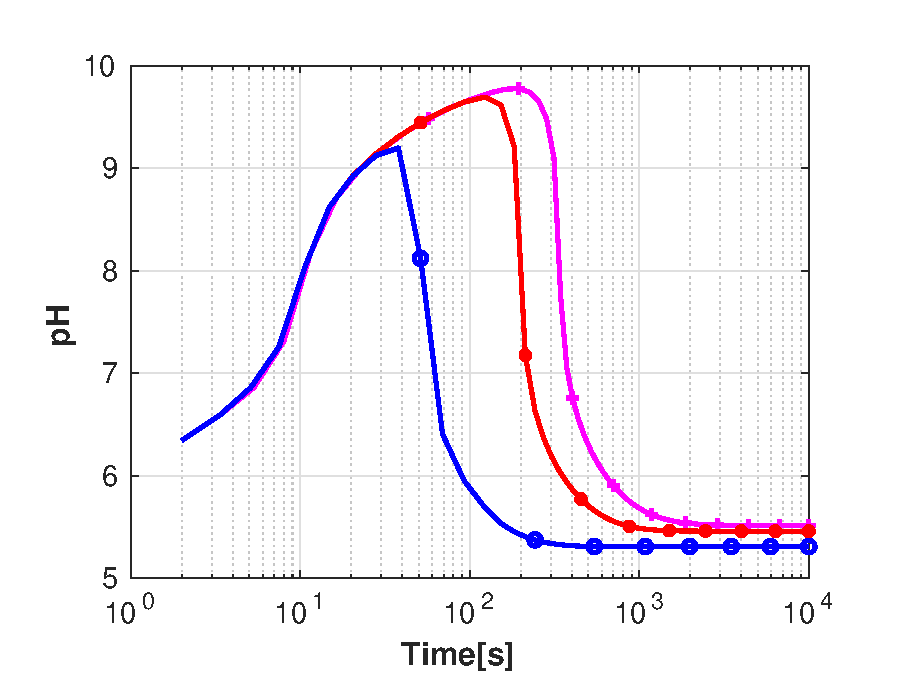
\includegraphics[width=\textwidth]{PICTURES/with_vel_pH.eps}
        \caption{Change in pH}
        \label{fig:velpH}       % Give a unique label
    \end{subfigure}%
        \hfill
        % here was an empty line which caused that the plots where not next
        % to each other but on top of each other
    \begin{subfigure}{.5\linewidth}
        \centering
        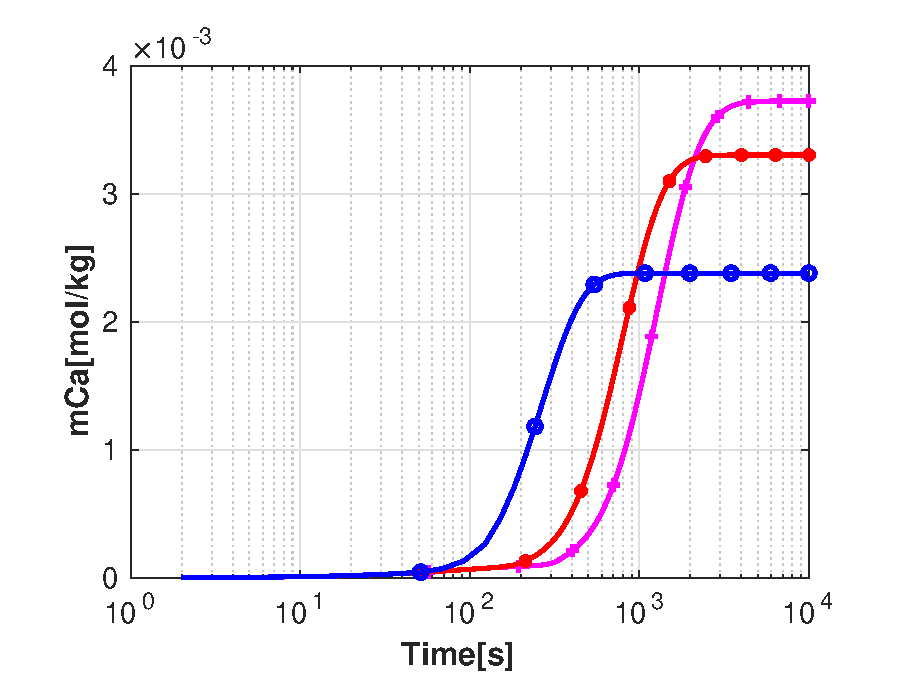
\includegraphics[width=\textwidth]{PICTURES/with_vel_mCa.eps}
        \caption{Change in molality of calcium (mCa)}
        \label{fig:velmCa}       % Give a unique label
    \end{subfigure}%
        \hfill
    \begin{subfigure}{.5\linewidth}
        \centering
        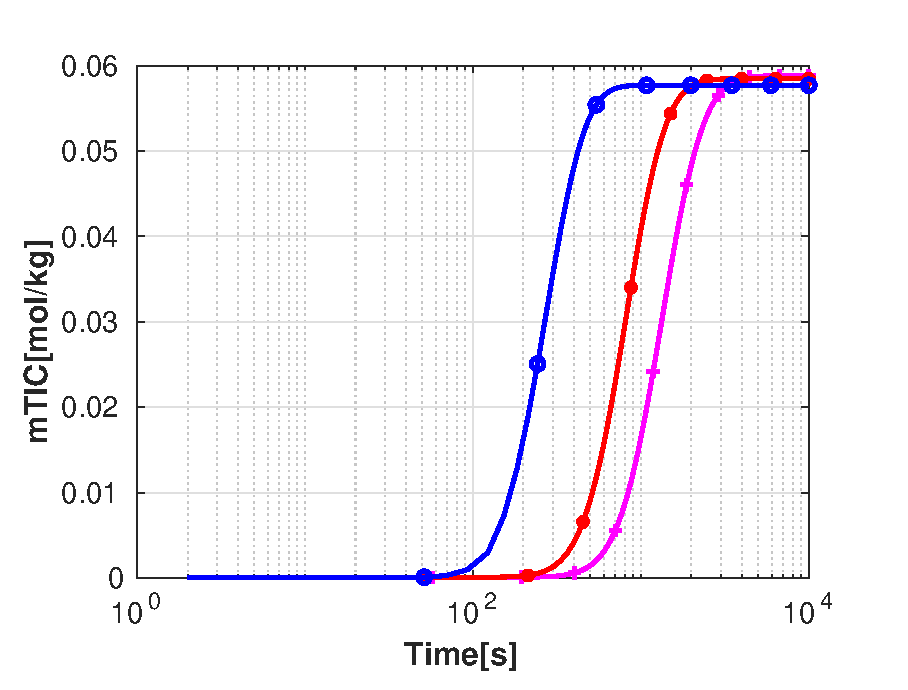
\includegraphics[width=\textwidth]{PICTURES/with_vel_mTIC.eps}
        \caption{Change in molality of total inorganic carbon (mTIC)}
        \label{fig:velmTIC}
    \end{subfigure}%
    \hfill
    \begin{subfigure}{.5\linewidth}
        \centering
        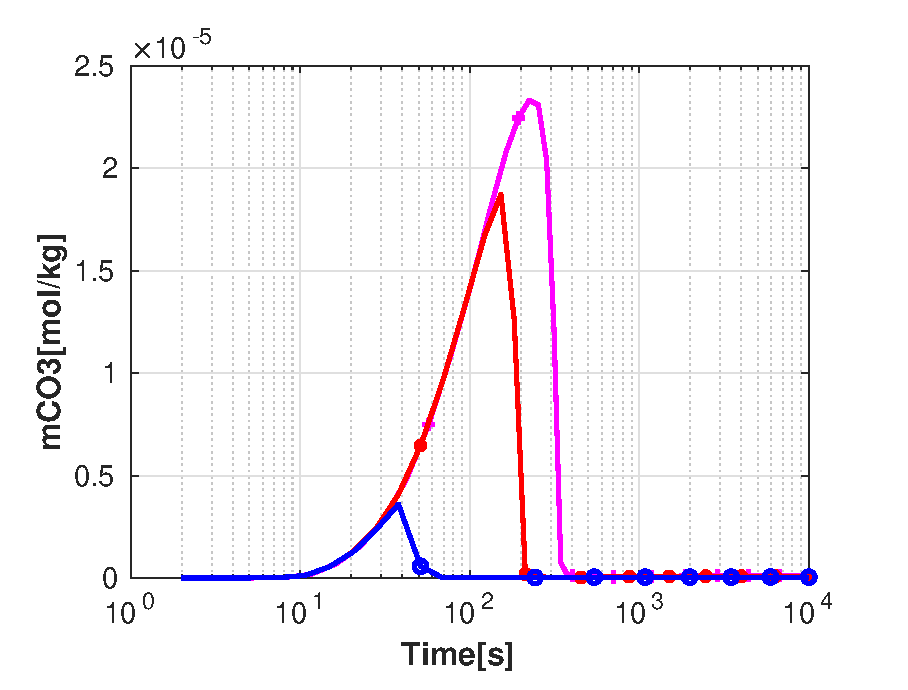
\includegraphics[width=\textwidth]{PICTURES/with_vel_mCO3.eps}
        \caption{Change in molality of carbonate (mCO3)}
        \label{fig:velmCO3}
    \end{subfigure}%
    \hfill
    \begin{subfigure}{.5\linewidth}
        \centering
        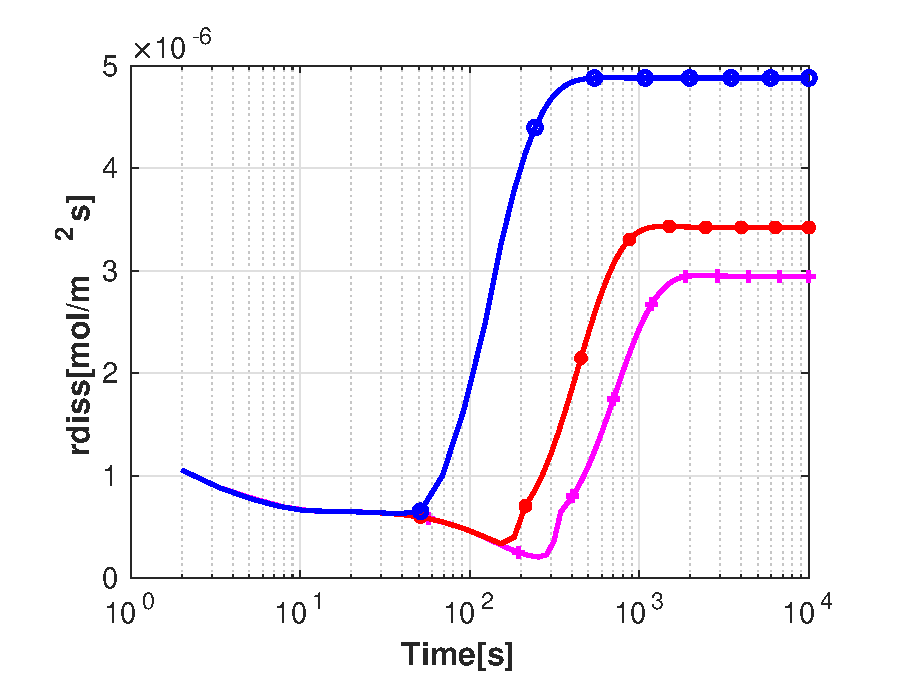
\includegraphics[width=\textwidth]{PICTURES/with_vel_rdiss.eps}
        \caption{Change in rate of dissolution of calcite (rdiss)}
        \label{fig:velrdiss}
    \end{subfigure}%
    \begin{subfigure}{.5\linewidth}
        \centering
        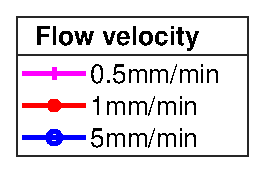
\includegraphics[width=0.40\textwidth]{PICTURES/with_vel_legend.eps}
        \caption{Legend}
        \label{fig:vellegend}
    \end{subfigure}%
    \hfill
     \caption{\DuMuX results that show the change in pH (\cref{fig:velpH}), molality of calcium (\cref{fig:velmCa}), 
     molality of total inorganic carbon (\cref{fig:velmTIC}), molality of carbonate (\cref{fig:velmCO3}) and rate of 
     dissolution of calcite (\cref{fig:velrdiss}) in time for different flow velocities in an open system}
     \label{fig:comparisionDiffFlowVelocity}
\end{figure}

The plots shown in figure \ref{fig:comparisionDiffFlowVelocity} is obtained for a cell at the boundary wall. 
All of the subplots, i.e., \subref{fig:1mmpermin}, \subref{fig:5mmpermin} and \subref{fig:0.5mmpermin}, 
show pH rises over time, reaches to its peak, and then descends to a steady-state value. The peak value 
varies with different initial and boundary conditions setups. 
The initial concentration of \code{TIC} i.e. 2.5e-7 [mol/mol] in the system is lower than the 
boundary condition i.e. 9.9956e-4 [mol/mol]. This leads to a low buffering capacity of the solution at the 
beginning, and with the incoming \ce{CO2} having higher concentration, pH rises rapidly. As time passes, 
the dissolved calcium-carbonate is transported away from the system and hence pH lowers and reaches a steady-state value.\\
Considering all the parameters to be constant, with the increase in flow-velocity the maximum pH decreases and system stabilizes faster. 
The reason is with faster transport of increased TIC, which is due to additional \ce{CO2} transported into the system and 
dissolved calcium-carbonate because of the reaction at the wall, out of the system due to higher flow velocity. 
Had there been initial and boundary conditions, we would not expect this peak to occur. It is because of the inconsistent 
BCs with the initial conditions that lead to this phenomenon. Since, we are mainly checking the plausibility of the model, 
we did not consider in defining a consistent BCs and initial conditions. A detail explanation to this phenomena and its dependency 
on initial and boundary conditions are discussed in subsection \ref{ssec:diffInitialBC}.


\subsubsection*{Different initial pH} \label{ssec:diffpH}
We fixed the flow-velocity to 1mm/min, did not include grid grading parameters, initial \ce{CO2} concentration was fixed to 2.5e-7[mol/mol] and boundary concentration at the top was set to 9.9956e-4[mol/mol]; just the initial pH at the start of the simulation were varied.

\begin{figure}[!h]
        \centering
    \begin{subfigure}{.5\linewidth}
            \centering
        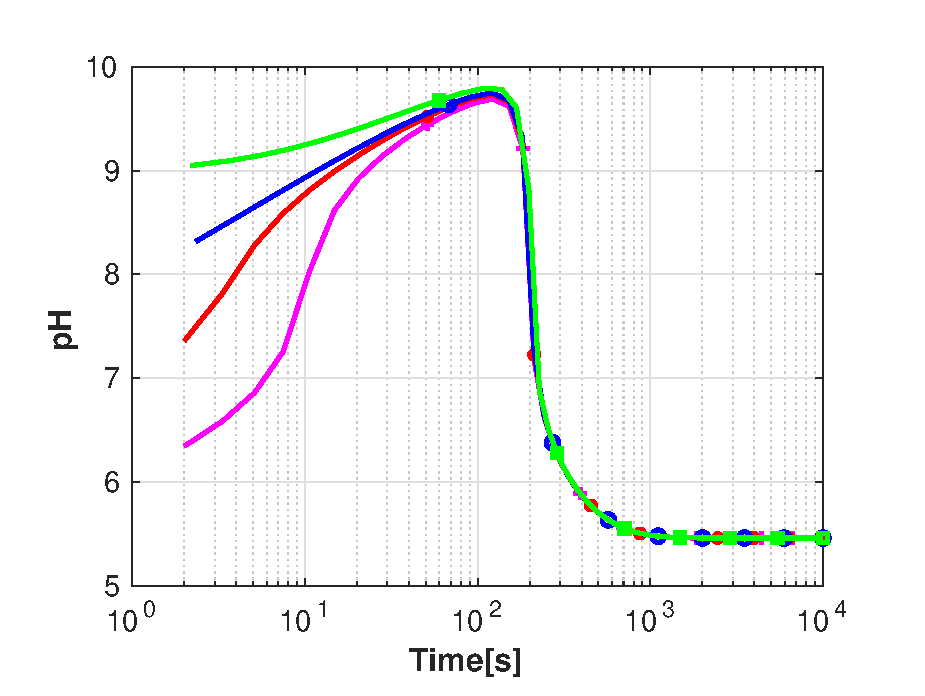
\includegraphics[width=\textwidth]{PICTURES/with_pH_pH.eps}
        \caption{Change in pH}
        \label{fig:pHpH}
    \end{subfigure}%
        \hfill
    \begin{subfigure}{.5\linewidth}
            \centering
        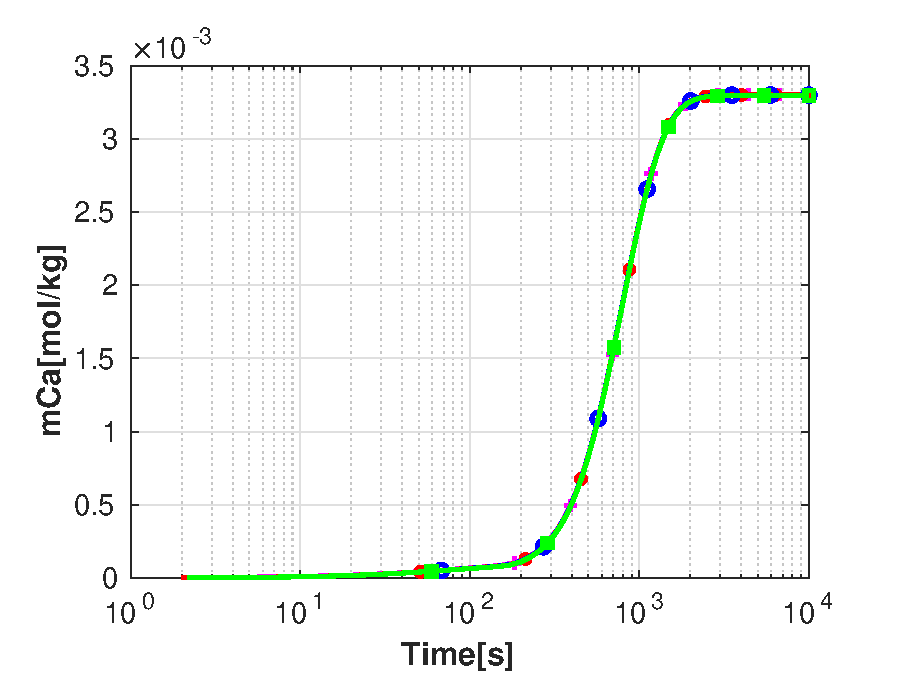
\includegraphics[width=\textwidth]{PICTURES/with_pH_mCa.eps}
        \caption{Change in molality of calcium (mCa)}
        \label{fig:pHmCa}
    \end{subfigure}%
    \hfill
    \begin{subfigure}{.5\linewidth}
            \centering
        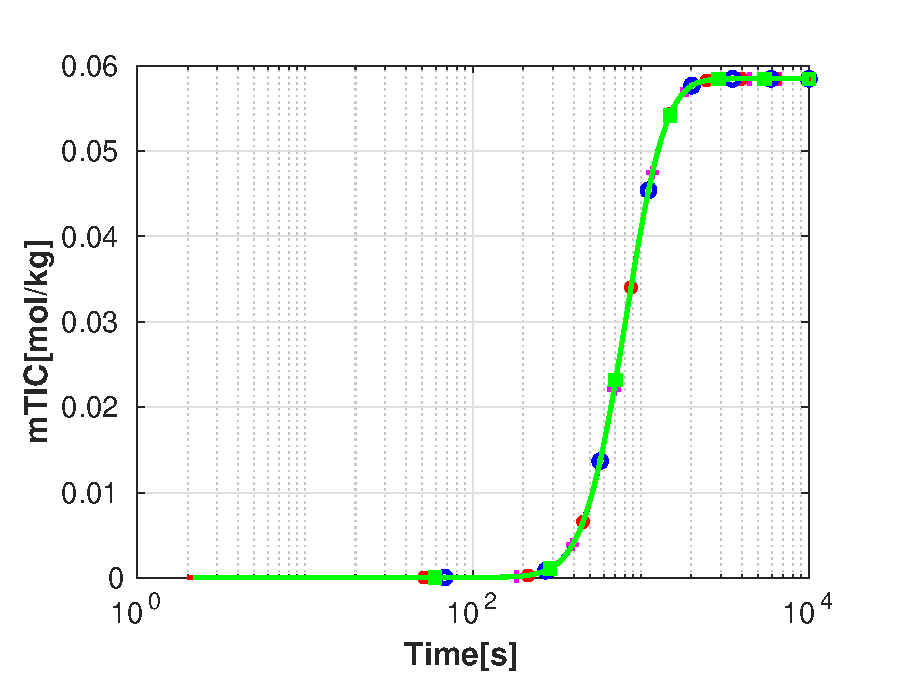
\includegraphics[width=\textwidth]{PICTURES/with_pH_mTIC.eps}
        \caption{Change in molality of total inorganic carbon (mTIC)}
        \label{fig:pHmTIC}
    \end{subfigure}%
    \hfill
    \begin{subfigure}{.5\linewidth}
            \centering
        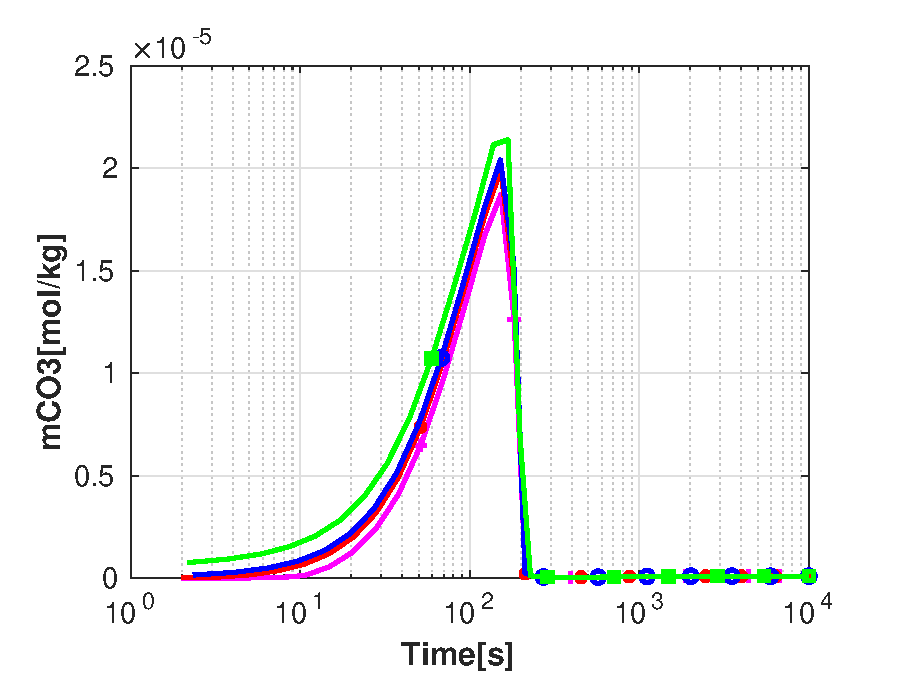
\includegraphics[width=\textwidth]{PICTURES/with_pH_mCO3.eps}
        \caption{Change in molality of carbonate (mCO3)}
        \label{fig:pHmCO3}
    \end{subfigure}%
    \hfill
    \begin{subfigure}{.5\linewidth}
            \centering
        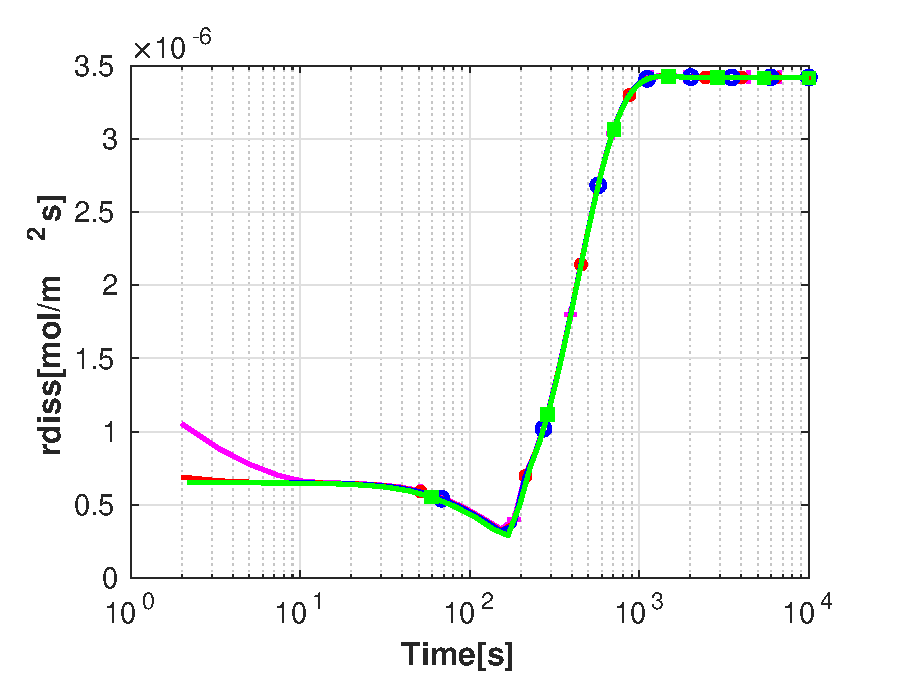
\includegraphics[width=\textwidth]{PICTURES/with_pH_rdiss.eps}
        \caption{Change in rate of dissolution of calcite (rdiss)}
        \label{fig:pHrdiss}
    \end{subfigure}%
  \hfill
  \begin{subfigure}{.5\linewidth}
            \centering
        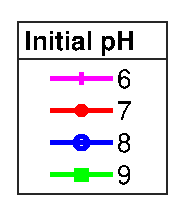
\includegraphics[width=0.25\textwidth]{PICTURES/with_pH_legend.eps}
        \caption{Legend}
        \label{fig:pHlegend}
    \end{subfigure}%
    \caption{\DuMuX results that show the change in pH (\cref{fig:pHpH}), molality of calcium (\cref{fig:pHmCa}), 
    molality of total inorganic carbon (\cref{fig:pHmTIC}), molality of carbonate (\cref{fig:pHmCO3}) and rate of 
    dissolution of calcite (\cref{fig:pHrdiss}) in time for different initial pH in an open system}
    \label{fig:comparisionDiffInitialpH}
\end{figure}


The figure \ref{fig:comparisionDiffInitialpH} shows pH rises over time, reaches to its peak, and then descends to a steady-state value, as seen on figure \ref{fig:comparisionDiffFlowVelocity}. The explanation for such phenomena holds true here as well. Increasing the initial pH also increases the steady-state pH. The time for system to be in steady-state is fairly same for all the cases, as expected. Since, this depends on the flow-velocity and initial and boundary concentration of \ce{CO2}, which is constant for all the cases. 

\subsubsection*{Different initial and boundary \ce{CO2} concentrations} \label{ssec:diffInitialBC}
We fixed the flow-velocity to 1mm/min, did not include grid grading and initial pH was set to 6.0; just the boundary condition at the top of the domain was varied to analyse the buffering effect in the pH growth of the water, keeping a constant initial concentration of \ce{CO2} inside the domain to be 2.5e-7 [mol/mol].

\begin{figure}[!h]
        \centering
    \begin{subfigure}{.5\linewidth}
            \centering
        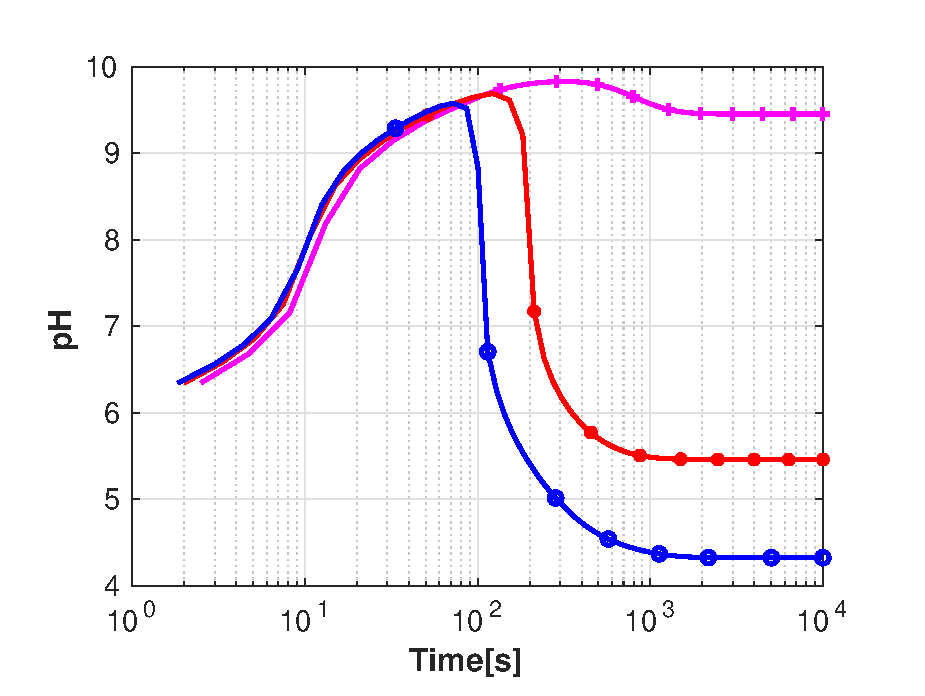
\includegraphics[width=\textwidth]{PICTURES/with_CO2_pH.eps}
        \caption{Change in pH}
        \label{fig:CO2pH}
    \end{subfigure}%
        \hfill
    \begin{subfigure}{.5\linewidth}
            \centering
        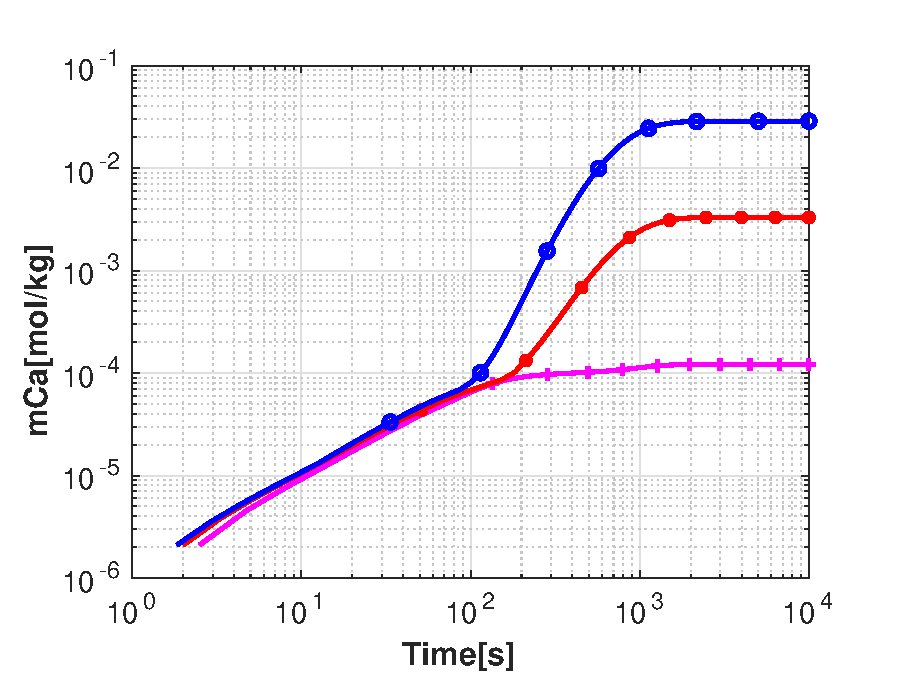
\includegraphics[width=\textwidth]{PICTURES/with_CO2_mCa.eps}
        \caption{Change in molality of calcium (mCa)}
        \label{fig:CO2mCa}
    \end{subfigure}%
        \hfill
    \begin{subfigure}{.5\linewidth}
            \centering
        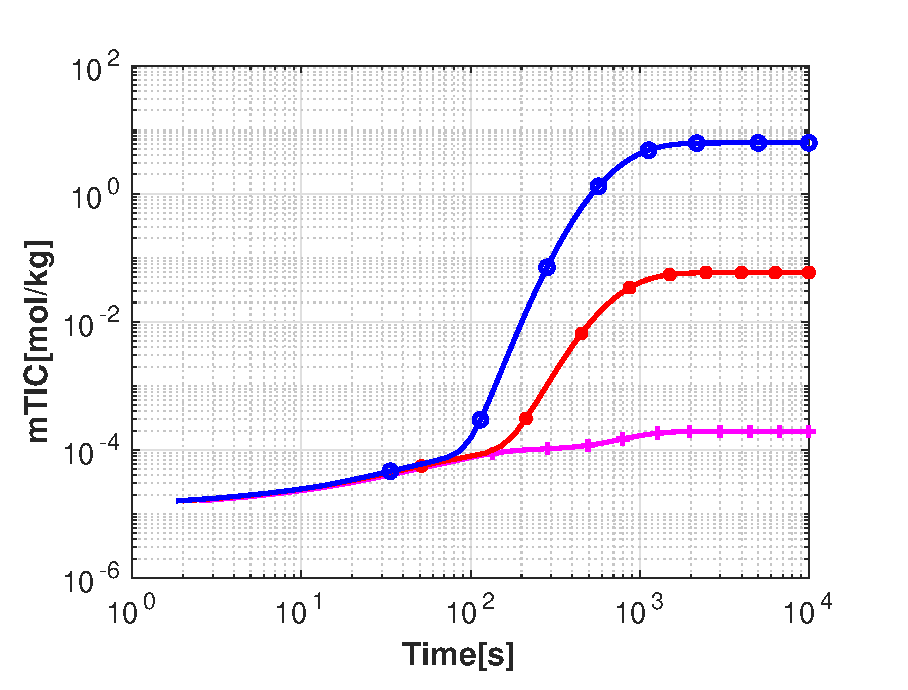
\includegraphics[width=\textwidth]{PICTURES/with_CO2_mTIC.eps}
        \caption{Change in molality of total inorganic carbon (mTIC)}
        \label{fig:CO2mTIC}
    \end{subfigure}%
    \hfill
    \begin{subfigure}{.5\linewidth}
            \centering
        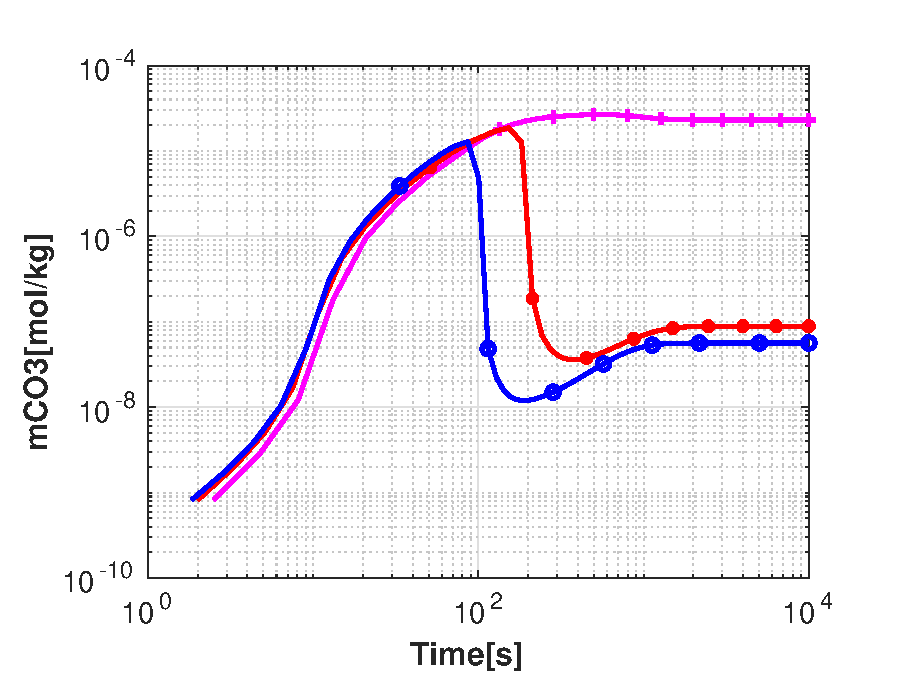
\includegraphics[width=\textwidth]{PICTURES/with_CO2_mCO3.eps}
        \caption{Change in molality of carbonate (mCO3)}
        \label{fig:CO2mCO3}
    \end{subfigure}%
    \hfill
    \begin{subfigure}{.5\linewidth}
            \centering
        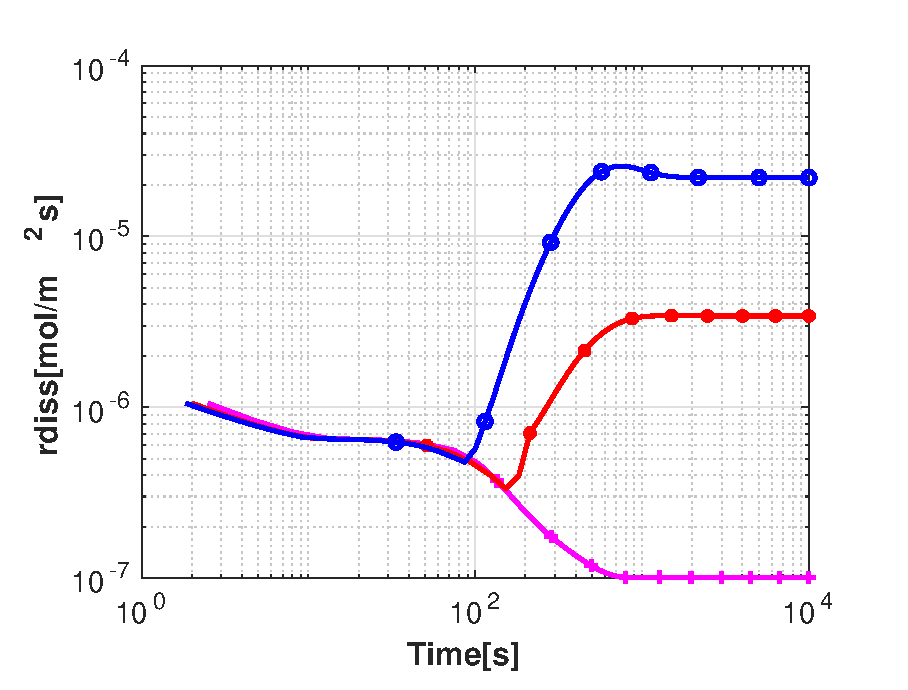
\includegraphics[width=\textwidth]{PICTURES/with_CO2_rdiss.eps}
        \caption{Change in rate of dissolution of calcite (rdiss)}
        \label{fig:CO2rdiss}
    \end{subfigure}%
    \hfill
    \begin{subfigure}{.5\linewidth}
            \centering
        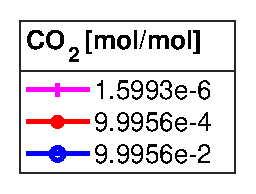
\includegraphics[width=0.35\textwidth]{PICTURES/with_CO2_legend.eps}
        \caption{Legend}
        \label{fig:CO2legend}
    \end{subfigure}%
    \caption{\DuMuX results that show the change in pH (\cref{fig:CO2pH}), molality of calcium (\cref{fig:CO2mCa}), molality of total inorganic carbon (\cref{fig:CO2mTIC}), molality of carbonate (\cref{fig:CO2mCO3}) and rate of dissolution of calcite (\cref{fig:CO2rdiss}) in time for different \ce{CO2} concentration at the top of the domain in an open system}
    \label{fig:diffCO2}
\end{figure}

The figure \ref{fig:diffCO2} shows the same rise in pH, with same pattern, over time. The difference now is the maximum pH and the steady-state pH value; the steady-state time is once again similar for all the subplots in fig. \ref{fig:CO2}. Decreasing the \ce{CO2} concentration at the top, but it still has a higher \ce{CO2} concentration than what's inside, as shown in fig. \subref{fig:CO2low}, shows the system is more or less consistent with the inside and incoming \ce{CO2}-enriched water. The pH rises steadily and reaches a peak, and without descending, stabilizes around same steady-state value. The dissolution capacity of water has not changed much throughout the simulation.\\
On the other hand, figure \subref{fig:CO2high} shows the same pattern as in figure \ref{fig:CO2} with a different peak and steady-state pH. The incoming water has higher \ce{CO2} concentration which mixes/replaces the lower \ce{CO2}-enriched water. Because of \ce{CO2}, reaction advances and hence pH rises, but as the simulation proceeds, the lower \ce{CO2}-enriched water with low buffering capacity is being replaced by water with high buffering capacity. Hence, the rise in pH is subdued and the pH falls until it reaches steady-state. 


\subsubsection*{Different Grid grading parameter} \label{ssec:diffGrid}
We fixed the initial pH to 6.0, flow-velocity to 1mm/min, initial \ce{CO2} was fixed to 2.5e-7[mol/mol] and at the boundary it was 9.9956e-4[mol/mol]; just the grid grading parameter was varied to properly resolve the boundary layer formation on the wall. We expect a boundary layer formation on the reactive wall in a cave scenario, but given the size of the domain we have, we were not able to see any difference in output values with and without grid-grading parameters. \\
We decreased the spacing of the grids near the wall in x-direction. We ran the simulation for grid-grading values 1.1 and 1.2.

\begin{figure}[!h]
        \centering
    \begin{subfigure}{.5\linewidth}
            \centering
        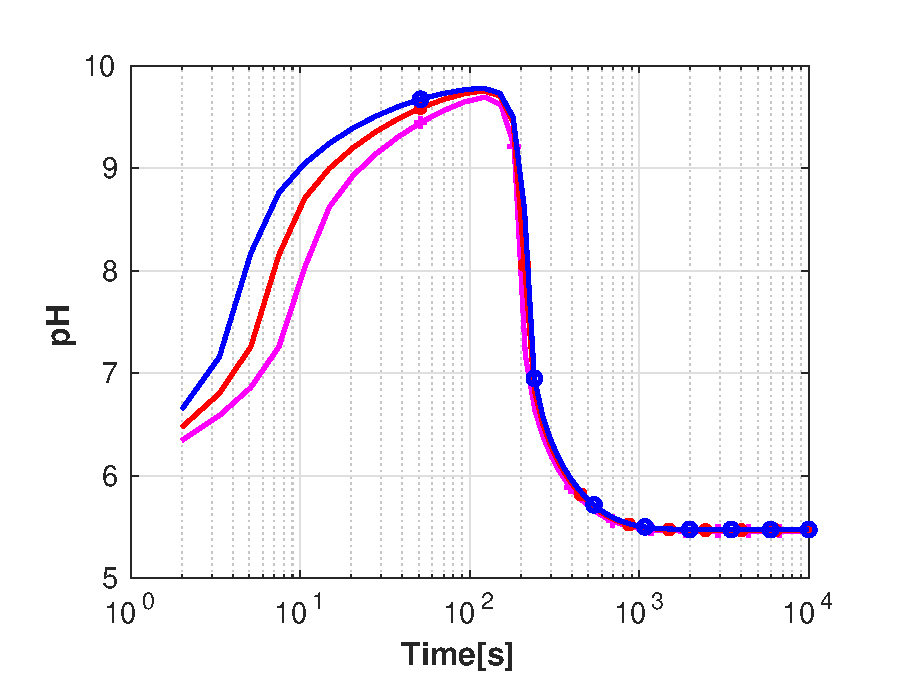
\includegraphics[width=\textwidth]{PICTURES/with_grid_pH.eps}
        \caption{Change in pH}
        \label{fig:gridpH}
    \end{subfigure}%
        \hfill
    \begin{subfigure}{.5\linewidth}
            \centering
        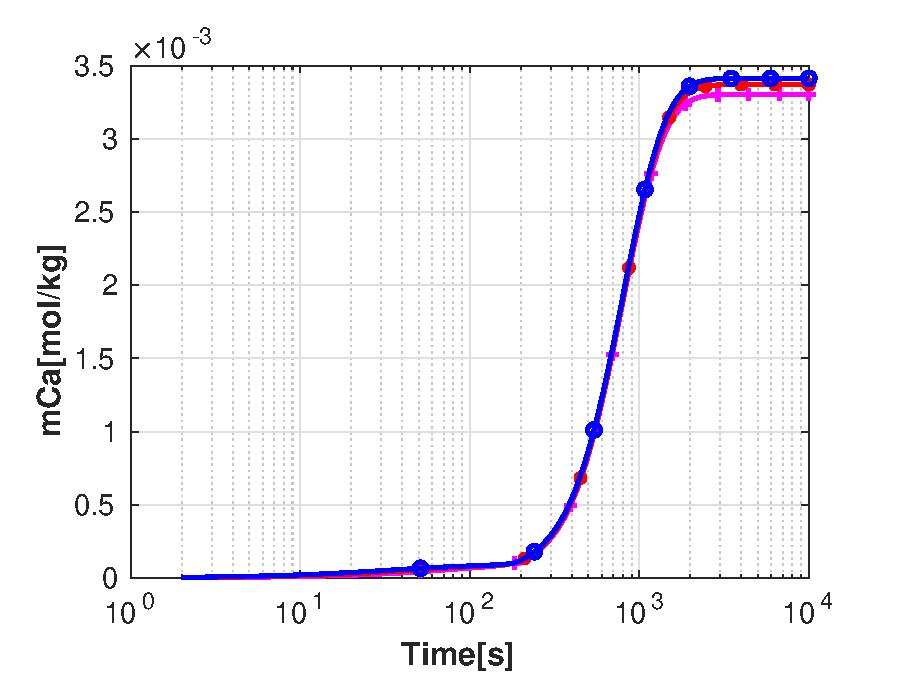
\includegraphics[width=\textwidth]{PICTURES/with_grid_mCa.eps}
        \caption{Change in molality of calcium (mCa)}
        \label{fig:gridmCa}
    \end{subfigure}%
        \hfill
        \begin{subfigure}{.5\linewidth}
            \centering
        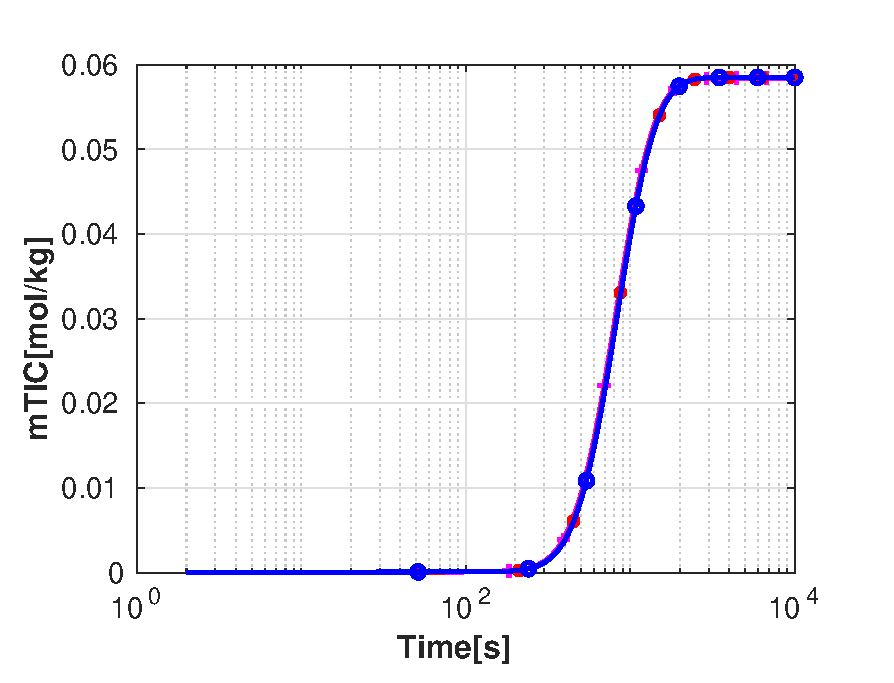
\includegraphics[width=\textwidth]{PICTURES/with_grid_mTIC.eps}
        \caption{Change in molality of total inorganic carbon (mTIC)}
        \label{fig:gridmTIC}
    \end{subfigure}%
        \hfill
        \begin{subfigure}{.5\linewidth}
            \centering
        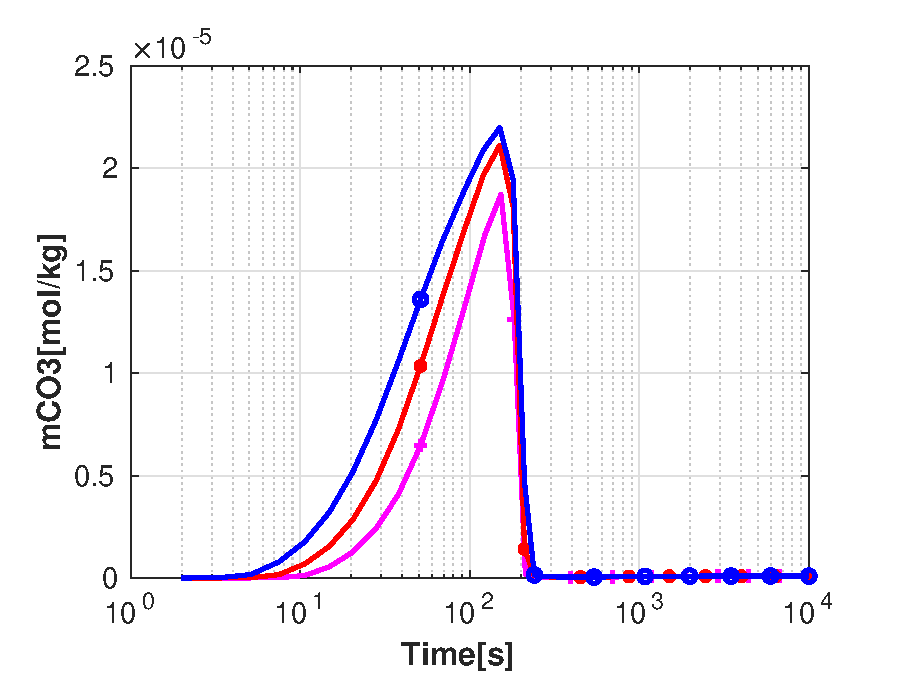
\includegraphics[width=\textwidth]{PICTURES/with_grid_mCO3.eps}
        \caption{Change in molality of carbonate (mCO3)}
        \label{fig:gridmCO3}
    \end{subfigure}%
        \hfill
        \begin{subfigure}{.5\linewidth}
            \centering
        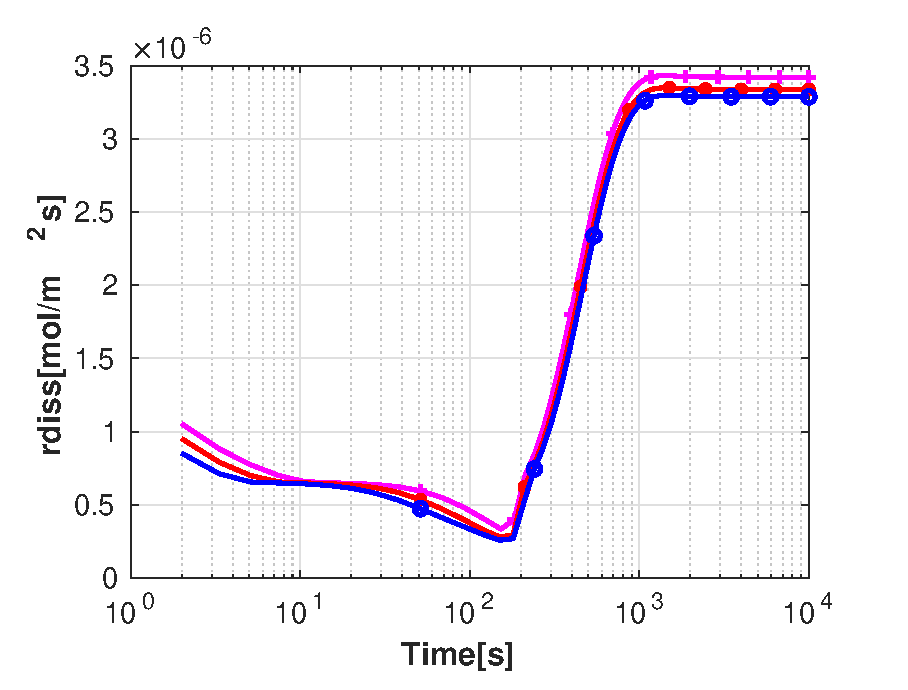
\includegraphics[width=\textwidth]{PICTURES/with_grid_rdiss.eps}
        \caption{Change in rate of dissolution of calcite (rdiss)}
        \label{fig:gridrdiss}
    \end{subfigure}%
        \hfill
        \begin{subfigure}{.5\linewidth}
            \centering
        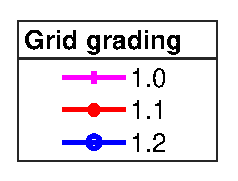
\includegraphics[width=0.35\textwidth]{PICTURES/with_grid_legend.eps}
        \caption{Legend}
        \label{fig:gridlegend}
    \end{subfigure}%
    \caption{\DuMuX results that show the change in pH (\cref{fig:gridpH}), molality of calcium (\cref{fig:gridmCa}), molality of total inorganic carbon (\cref{fig:gridmTIC}), molality of carbonate (\cref{fig:gridmCO3}) and rate of dissolution of calcite (\cref{fig:gridrdiss}) in time for different grid grading parameter in an open system}
    \label{fig:diffGrid}
\end{figure}

The reason we chose grid grading near the wall is to resolve the boundary layer developed on the wall. Since the model we chose was too small, we were inside the boundary layer and that was the reason why we did not see any differences in the subplots in the figure \ref{fig:diffGrid}.

\subsubsection*{Contour plots} \label{ssec:contour}
We fixed pH of the water to 6 and did not include grid grading parameters in the input file -- just the flow velocity was varied. We set the initial concentration of \ce{CO2} throughout the domain to be 2.5e-7 [mol\_\ce{CO2}/mol\_\ce{H2O}] and the boundary condition at the top of the domain to be 9.9956e-4 [mol/mol].


\paragraph*{pH contour plots} \mbox{}\\
% steady state pH
\begin{figure}[!h]
\centering
    \begin{subfigure}{.5\linewidth}
        \centering
        \includegraphics[trim=450 20 450 20, clip, width=0.9\textwidth]{PICTURES/contour_vel1mm_pH.eps}
        \caption{Flow Velocity = 1mm/min}
        \label{fig:pHSteady-state}       % Give a unique label
    \end{subfigure}%
    \hfill
    \begin{subfigure}{.5\linewidth}
        \centering
        \includegraphics[trim=450 20 450 20, clip, width=0.9\textwidth]{PICTURES/contour_vel5mm_pH.eps}
        \caption{Flow Velocity = 5mm/min}
        \label{fig:pHSteady-state5mm}       % Give a unique label
    \end{subfigure}%
    \hfill
    \begin{subfigure}{.5\linewidth}
        \centering
        \includegraphics[trim=450 20 450 20, clip, width=\textwidth]{PICTURES/contour_vel0.5mm_pH.eps}
        \caption{Flow Velocity = 0.5mm/min}
        \label{fig:pHSteady-state0.5mm}       % Give a unique label
    \end{subfigure}%
    \caption{\DuMuX Contour plots: Numerical results that show the distribution of pH at the steady-state in an open system}
     \label{fig:contourpH}
\end{figure}

Figure \ref{fig:contourpH} shows contour plots for pH at the steady-state in varying flow-velocities. All the subplots \ref{fig:pHSteady-state}, \ref{fig:pHSteady-state5mm}, \ref{fig:pHSteady-state0.5mm} show higher pH value near the reactive wall, and the pH decreases as we go away from the wall. The dissolved calcium-carbonate is diffused along the x-axis which causes the rise in pH adjacent to the reactive wall which fades out as we go away from the wall.


\paragraph*{mCO3 contour plots} \mbox{}\\

%steady-state CO3
\begin{figure}[!h]
\centering
    \begin{subfigure}{.5\linewidth}
        \centering
        \includegraphics[trim=450 20 450 20, clip, width=0.9\textwidth]{PICTURES/contour_vel1mm_mCO3.eps}
        \caption{Flow Velocity = 1mm/min}
        \label{fig:CO3Steady-state}       % Give a unique label
    \end{subfigure}%
    \hfill
    \begin{subfigure}{.5\linewidth}
        \centering
        \includegraphics[trim=450 20 450 20, clip, width=0.9\textwidth]{PICTURES/contour_vel5mm_mCO3.eps}
        \caption{Flow Velocity = 5mm/min}
        \label{fig:CO3Steady-state5mm}       % Give a unique label
    \end{subfigure}%
    \hfill
    \begin{subfigure}{.5\linewidth}
        \centering
        \includegraphics[trim=450 20 450 20, clip, width=0.9\textwidth]{PICTURES/contour_vel0.5mm_mCO3.eps}
        \caption{Flow Velocity = 0.5mm/min}
        \label{fig:CO3Steady-state0.5mm}       % Give a unique label
    \end{subfigure}%
    \caption{\DuMuX Contour plots: Numerical results that show the distribution of molality of carbonate at the steady-state in an open system}
     \label{fig:contourCO3}
\end{figure}


Figure \ref{fig:contourCO3} shows contour plots for the concentration of \ce{CO3}\textsuperscript{2-} at the steady-state in varying flow-velocities. All the subplots \ref{fig:CO3Steady-state}, \ref{fig:CO3Steady-state5mm}, \ref{fig:CO3Steady-state0.5mm} show a similar pattern: higher concentration near the reactive wall, where dissolution of calcium-carbonate is adding \ce{CO3}\textsuperscript{2-} into the karst water. As we go away from the wall, concentration of \ce{CO3}\textsuperscript{2-} starts to decrease -- the dissolved calcium-carbonate is diffused along the x-axis which causes a formation of concentration gradient along x-axis -- and reaches as far as the diffusion takes it. Had the simulation ran for longer times than for 6000s (the time we ran for this case), the contour would have migrated further to the right. 

\paragraph*{mTIC contour plots} \mbox{}\\
% steady state TIC
\begin{figure}[!h]
\centering
    \begin{subfigure}{.5\linewidth}
        \centering
        \includegraphics[trim=450 20 450 20, clip, width=0.9\textwidth]{PICTURES/contour_vel1mm_mTIC.eps}
        \caption{Flow Velocity = 1mm/min}
        \label{fig:TICSteady-state}       % Give a unique label
    \end{subfigure}%
    \hfill
    \begin{subfigure}{.5\linewidth}
        \centering
        \includegraphics[trim=450 20 450 20, clip, width=0.9\textwidth]{PICTURES/contour_vel5mm_mTIC.eps}
        \caption{Flow Velocity = 5mm/min}
        \label{fig:TICSteady-state5mm}       % Give a unique label
    \end{subfigure}%
    \hfill
    \begin{subfigure}{.5\linewidth}
        \centering
        \includegraphics[trim=450 20 450 20, clip, width=0.9\textwidth]{PICTURES/contour_vel0.5mm_mTIC.eps}
        \caption{Flow Velocity = 0.5mm/min}
        \label{fig:TICSteady-state0.5mm}       % Give a unique label
    \end{subfigure}%
    \caption{\DuMuX Contour plots: Numerical results that show the distribution of molality of total inorganic carbon at the steady-state in an open system}
     \label{fig:contourTIC}
\end{figure}

Figure \ref{fig:contourTIC} shows contour plots for concentration of Total Inorganic Carbon (TIC) at the steady-state in varying flow-velocities. All the subplots \ref{fig:TICSteady-state}, \ref{fig:TICSteady-state5mm}, \ref{fig:TICSteady-state0.5mm} show the system has more or less come to a steady-state. \ce{CO2} is carried into the system with the flow, which also gets diffused and gets mixed within the system as the time progresses, which causes the concentration to be fairly constant throughout the system. 


\paragraph*{mCa contour plots} \mbox{}\\

% steady state Ca
\begin{figure}[!h]
\centering
    \begin{subfigure}{.5\linewidth}
        \centering
        \includegraphics[trim=450 20 450 20, clip, width=0.9\textwidth]{PICTURES/contour_vel1mm_mCa.eps}
        \caption{Flow Velocity = 1mm/min}
        \label{fig:CaSteady-state}       % Give a unique label
    \end{subfigure}%
    \hfill
    \begin{subfigure}{.5\linewidth}
        \centering
        \includegraphics[trim=450 20 450 20, clip, width=0.9\textwidth]{PICTURES/contour_vel5mm_mCa.eps}
        \caption{Flow Velocity = 5mm/min}
        \label{fig:CaSteady-state5mm}       % Give a unique label
    \end{subfigure}%
    \hfill
    \begin{subfigure}{.5\linewidth}
        \centering
        \includegraphics[trim=450 20 450 20, clip, width=0.9\textwidth]{PICTURES/contour_vel0.5mm_mCa.eps}
        \caption{Flow Velocity = 0.5mm/min}
        \label{fig:CaSteady-state0.5mm}       % Give a unique label
    \end{subfigure}%
    \caption{\DuMuX Contour plots: Numerical results that show the distribution of molality of calcium at the steady-state in an open system}
     \label{fig:contourCa}
\end{figure}

Figure \ref{fig:contourCa} shows contour plots for concentration of Ca\textsuperscript{2+} at the steady-state in varying flow-velocities. All the subplots \ref{fig:CaSteady-state}, \ref{fig:CaSteady-state5mm}, \ref{fig:CaSteady-state0.5mm} show higher concentration near the reactive wall, and the concentration decreases as we go away from the wall. The dissolved calcium-carbonate is diffused along the x-axis which causes the rise in concentration of Ca\textsuperscript{2+} adjacent to the reactive wall which fades out as we go away from the wall.


\subsection{\DuMuX Simulation results: Closed system}
\subsubsection*{Different initial pH} \label{ssec:diffinitialpHnoflow}
The purpose of the simulation runs without flow-velocity was for the validation purpose with \MATLAB results. The initial concentration of \ce{CO2} in the karst water was set to 2.5e-7 [mol/mol]. We did not include grid grading parameters; the initial pH at the start of the simulation were varied.

\begin{figure}[!h]
        \centering
    \begin{subfigure}{.5\linewidth}
            \centering
        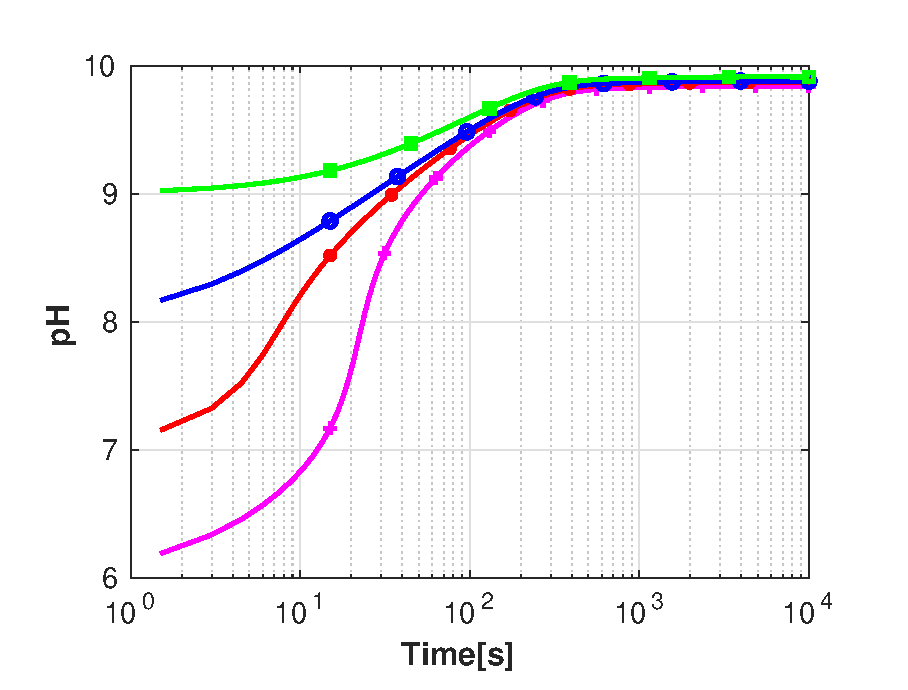
\includegraphics[width=\textwidth]{PICTURES/without_pH_pH.eps}
        \caption{Change in pH}
        \label{fig:withoutpHpH}
    \end{subfigure}%
        \hfill
    \begin{subfigure}{.5\linewidth}
            \centering
        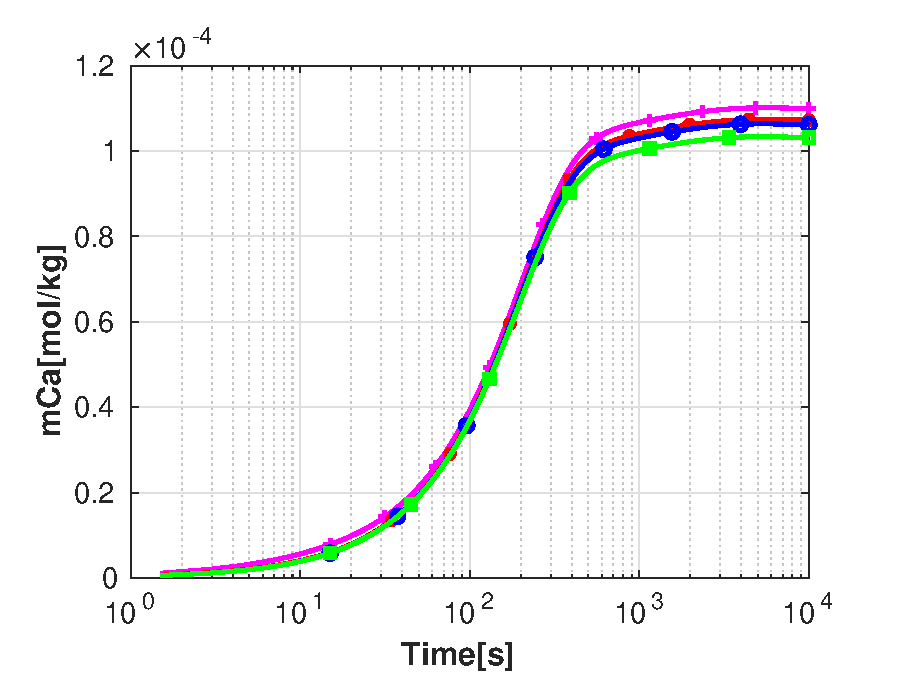
\includegraphics[width=\textwidth]{PICTURES/without_pH_mCa.eps}
        \caption{Change in molality of calcium (mCa)}
        \label{fig:withoutpHmCa}
    \end{subfigure}%
    \hfill
    \begin{subfigure}{.5\linewidth}
            \centering
        \includegraphics[width=\textwidth]{PICTURES/without_pH_mTIC.eps}
        \caption{Change in molality of total inorganic carbon (mTIC)}
        \label{fig:withoutpHmTIC}
    \end{subfigure}%
    \hfill
    \begin{subfigure}{.5\linewidth}
            \centering
        \includegraphics[width=\textwidth]{PICTURES/without_pH_mCO3.eps}
        \caption{Change in molality of carbonate (mCO3)}
        \label{fig:withoutpHmCO3}
    \end{subfigure}%
    \hfill
    \begin{subfigure}{.5\linewidth}
            \centering
        \includegraphics[width=\textwidth]{PICTURES/without_pH_rdiss.eps}
        \caption{Change in rate of dissolution of calcite (rdiss)}
        \label{fig:withoutpHrdiss}
    \end{subfigure}%
  \hfill
  \begin{subfigure}{.5\linewidth}
            \centering
        \includegraphics[width=0.25\textwidth]{PICTURES/with_pH_legend.eps}
        \caption{Legend}
        \label{fig:withoutpHlegend}
    \end{subfigure}%
    \caption{\DuMuX results that show the change in pH (\cref{fig:withoutpHpH}), molality of calcium (\cref{fig:withoutpHmCa}), molality of total inorganic carbon (\cref{fig:withoutpHmTIC}), molality of carbonate (\cref{fig:withoutpHmCO3}) and rate of dissolution of calcite (\cref{fig:withoutpHrdiss}) in time for different initial pH in a closed system}
    
    \label{fig:comparisionWithoutDiffInitialpH}
\end{figure}

The figure \ref{fig:diffInitialpHNoFlow}, for all the sub-plots, shows pH increases as the dissolution advances and after some time it reaches steady-state condition. Unlike a similar scenario with flow-velocity, as shown in figure \ref{fig:comparisionDiffInitialpH}, there is no descend curve. The reasons are: there is no flow-velocity to transport the dissolved calcium-carbonate out of the system, and the karst water is not in contact with the outer environment, hence there is no transport of TIC into the karst water, which means there is no rapid increase in pH and no descend curve, rather pH increases constructively and stabilizes to a steady-state value.


\subsubsection*{Different Grid grading parameter} \label{ssec:diffGridnoflow}
We fixed the initial pH in the karst water to 6.0 and the initial concentration of \ce{CO2}  was set to 2.5e-7 [mol/mol]. We decreased the spacing of the grids near the wall in x-direction. We ran the simulation for grid-grading values 1.1 and 1.2. 

\begin{figure}[!h]
        \centering
    \begin{subfigure}{.5\linewidth}
            \centering
        \includegraphics[width=\textwidth]{PICTURES/without_grid_pH.eps}
        \caption{Change in pH}
        \label{fig:withoutgridpH}
    \end{subfigure}%
        \hfill
    \begin{subfigure}{.5\linewidth}
            \centering
        \includegraphics[width=\textwidth]{PICTURES/without_grid_mCa.eps}
        \caption{Change in molality of calcium (mCa)}
        \label{fig:withoutgridmCa}
    \end{subfigure}%
    \hfill
    \begin{subfigure}{.5\linewidth}
            \centering
        \includegraphics[width=\textwidth]{PICTURES/without_grid_mTIC.eps}
        \caption{Change in molality of total inorganic carbon (mTIC)}
        \label{fig:withoutgridmTIC}
    \end{subfigure}%
    \hfill
    \begin{subfigure}{.5\linewidth}
            \centering
        \includegraphics[width=\textwidth]{PICTURES/without_grid_mCO3.eps}
        \caption{Change in molality of carbonate (mCO3)}
        \label{fig:withoutgridmCO3}
    \end{subfigure}%
    \hfill
    \begin{subfigure}{.5\linewidth}
            \centering
        \includegraphics[width=\textwidth]{PICTURES/without_grid_rdiss.eps}
        \caption{Change in rate of dissolution of calcite (rdiss)}
        \label{fig:withoutgridrdiss}
    \end{subfigure}%
  \hfill
  \begin{subfigure}{.5\linewidth}
            \centering
        \includegraphics[width=0.35\textwidth]{PICTURES/with_grid_legend.eps}
        \caption{Legend}
        \label{fig:withoutgridlegend}
    \end{subfigure}%
    \caption{\DuMuX results that show the change in pH (\cref{fig:withoutgridpH}), molality of calcium (\cref{fig:withoutgridmCa}), molality of total inorganic carbon (\cref{fig:withoutgridmTIC}), molality of carbonate (\cref{fig:withoutgridmCO3}) and rate of dissolution of calcite (\cref{fig:withoutgridrdiss}) in time for different grid grading parameter in a closed system} 
    \label{fig:comparisionWithoutDiffgrid}
\end{figure}


\begin{figure}[!h]The sub-figures \subref{fig:Noflowgrid1.1} and \subref{fig:Noflowgrid1.2} in the figure \ref{ssec:diffGridnoflow} did not show any differences. The reason is the same as explained in subsection \ref{ssec:diffGrid}.

\section{\MATLAB Simulation results}

        \centering
    \begin{subfigure}{.5\linewidth}
        \centering
        \includegraphics[width=\textwidth]{PICTURES/without_vel_pH.eps}
        \caption{Change in pH}
        \label{fig:withoutvelpH}       % Give a unique label
    \end{subfigure}%
        \hfill
        % here was an empty line which caused that the plots where not next
        % to each other but on top of each other
    \begin{subfigure}{.5\linewidth}
        \centering
        \includegraphics[width=\textwidth]{PICTURES/without_vel_mCa.eps}
        \caption{Change in molality of calcium (mCa)}
        \label{fig:withoutvelmCa}       % Give a unique label
    \end{subfigure}%
        \hfill
    \begin{subfigure}{.5\linewidth}
        \centering
        \includegraphics[width=\textwidth]{PICTURES/without_vel_mTIC.eps}
        \caption{Change in molality of total inorganic carbon (mTIC)}
        \label{fig:withoutvelmTIC}
    \end{subfigure}%
    \hfill
    \begin{subfigure}{.5\linewidth}
        \centering
        \includegraphics[width=\textwidth]{PICTURES/without_vel_mCO3.eps}
        \caption{Change in molality of carbonate (mCO3)}
        \label{fig:withoutvelmCO3}
    \end{subfigure}%
    \hfill
    \begin{subfigure}{.5\linewidth}
        \centering
        \includegraphics[width=\textwidth]{PICTURES/without_vel_rdiss.eps}
        \caption{Change in rate of dissolution of calcite (rdiss)}
        \label{fig:withoutvelrdiss}
    \end{subfigure}%
    \hfill
    \begin{subfigure}{.5\linewidth}
        \centering
        \includegraphics[width=0.25\textwidth]{PICTURES/with_pH_legend.eps}
        \caption{Legend}
        \label{fig:withoutvellegend}
    \end{subfigure}%
     \caption{\MATLAB results that show the change in pH (\cref{fig:withoutvelpH}), molality of calcium (\cref{fig:withoutvelmCa}), molality of total inorganic carbon (\cref{fig:withoutvelmTIC}), molality of carbonate (\cref{fig:withoutvelmCO3}) and rate of dissolution of calcite (\cref{fig:withoutvelrdiss}) in time for different initial pH in a closed system of 2D volume [15mm $\times$ 5mm]}
     \label{fig:MATLABcomparisionDiffInitialpH}
\end{figure}


\section{Comparison \DuMuX and \MATLAB} \label{sec:dvm}

\begin{table}[ht]
\small\addtolength{\tabcolsep}{-12pt}
\centering
\caption{\DuMuX and \MATLAB comparison table that lists steady-state time, pH, molality of calcium (mCa), molality of total inorganic carbon (mTIC) and molality of carbonate (mCO3) for a closed system of size 15mm$\times$5mm with varying initial pH, reactive area and batch volume}
\begin{tabular}{|c|c|c|c|c|c|c|c|c|c|c|c|c|}
    \hline
    \thead{Initial \\pH} & \thead{Reactive \\area} & \thead{Batch \\Volume} & \multicolumn{5}{c|}{\thead{Steady-state \MATLAB}} & \multicolumn{5}{c|}{\thead{Steady-state \DuMuX}} \\
    \cline{4-13}
    & & & \thead{time} & \thead{pH} & \thead{mCa}      & \thead{mTIC}     & \thead{mCO3}     & \thead{time} & \thead{pH} & \thead{mCa}      & \thead{mTIC}     & \thead{mCO3}\\
    & mm & \ce{mm^2} &  [s]  & [-] & [mol/kg] & [mol/kg] & [mol/kg] & [s] & [-]   & [mol/kg] & [mol/kg] & [mol/kg]\\
    \hline
    % initial pH   Reactive area Batch Volume time pH mCa mTIC mCO3 time pH mCa mTIC mCO3
      & 5  & 5   & 321  & 9.83 & 1.09e-4 & 1.23e-4 & 3.01e-5 & 321 & 9.83 & 1.09e-4 & 1.23e-4 & 3.01e-5 \\
    6 & 15 & 75  & 1601 & 9.83 & 1.09e-4 & 1.23e-4 & 3.01e-5 & 1596 & 9.83 & 1.09e-4 & 1.23e-4 & 3.01e-5 \\
      & 30 & 300 & 3201 & 9.83 & 1.09e-4 & 1.23e-4 & 3.01e-5 & 3190 & 9.83 & 1.09e-4 & 1.23e-4 & 3.01e-5 \\
    \hline
      & 5  & 5   & 331  & 9.86 & 1.06e-4 & 1.20e-4 & 3.09e-5 & 338  & 9.86 & 1.06e-4 & 1.20e-4 & 3.09e-5 \\
    7 & 15 & 75  & 1701 & 9.86 & 1.06e-4 & 1.20e-4 & 3.09e-5 & 1679 & 9.86 & 1.06e-4 & 1.20e-4 & 3.09e-5 \\
      & 30 & 300 & 3301 & 9.86 & 1.06e-4 & 1.20e-4 & 3.09e-5 & 3357 & 9.86 & 1.06e-4 & 1.20e-4 & 3.09e-5 \\
    \hline
      & 5  & 5   & 321  & 9.87 & 1.05e-4 & 1.19e-4 & 3.12e-5 & 324  & 9.87 & 1.05e-4 & 1.19e-4 & 3.12e-5 \\
    8 & 15 & 75  & 1701 & 9.87 & 1.05e-4 & 1.19e-4 & 3.12e-5 & 1610 & 9.87 & 1.05e-4 & 1.19e-4 & 3.12e-5 \\
      & 30 & 300 & 3201 & 9.87 & 1.05e-4 & 1.19e-4 & 3.12e-5 & 3219 & 9.87 & 1.05e-4 & 1.19e-4 & 3.12e-5 \\
    \hline
      & 5  & 5   & 611  & 9.91 & 1.02e-4 & 1.16e-4 & 3.21e-5 & 294  & 9.90 & 1.02e-4 & 1.16e-4 & 3.21e-5 \\
    9 & 15 & 75  & 3001 & 9.91 & 1.02e-4 & 1.16e-4 & 3.21e-5 & 1463 & 9.90 & 1.02e-4 & 1.16e-4 & 3.21e-5 \\
      & 30 & 300 & 6101 & 9.91 & 1.02e-4 & 1.16e-4 & 3.21e-5 & 2924 & 9.90 & 1.02e-4 & 1.16e-4 & 3.21e-5 \\
    \hline
\end{tabular}
% \end{adjustbox}
\label{tab:DumuxVsMatlab}
\end{table}


\begin{figure}[!h]
        \centering
    \begin{subfigure}{.5\linewidth}
            \centering
        \includegraphics[width=\textwidth]{PICTURES/dvm_pH6_pH.eps}
        \caption{Change in pH}
        \label{fig:dvmpH6pH}
    \end{subfigure}%
        \hfill
    \begin{subfigure}{.5\linewidth}
            \centering
        \includegraphics[width=\textwidth]{PICTURES/dvm_pH6_mCa.eps}
        \caption{Change in molality of calcium (mCa)}
        \label{fig:dvmpH6mCa}
    \end{subfigure}%
    \hfill
    \begin{subfigure}{.5\linewidth}
            \centering
        \includegraphics[width=\textwidth]{PICTURES/dvm_pH6_mTIC.eps}
        \caption{Change in molality of total inorganic carbon (mTIC)}
        \label{fig:dvmpH6mTIC}
    \end{subfigure}%
    \hfill
    \begin{subfigure}{.5\linewidth}
            \centering
        \includegraphics[width=\textwidth]{PICTURES/dvm_pH6_mCO3.eps}
        \caption{Change in molality of carbonate (mCO3)}
        \label{fig:dvmpH6mCO3}
    \end{subfigure}%
    \hfill
    \begin{subfigure}{.5\linewidth}
            \centering
        \includegraphics[width=\textwidth]{PICTURES/dvm_pH6_rdiss.eps}
        \caption{Change in rate of dissolution of calcite (rdiss)}
        \label{fig:dvmpH6rdiss}
    \end{subfigure}%
  \hfill
  \hfill
    \begin{subfigure}{.5\linewidth}
            \centering
        \includegraphics[width=0.85\textwidth]{PICTURES/dvm_pH6_legend.eps}
        \caption{Legend}
        \label{fig:dvmpH6legend}
    \end{subfigure}%
    \caption{Comparison: \DuMuX and \MATLAB results that show the change in pH (\cref{fig:dvmpH6pH}), molality of calcium (\cref{fig:dvmpH6mCa}), molality of total inorganic carbon (\cref{fig:dvmpH6mTIC}), molality of carbonate (\cref{fig:dvmpH6mCO3}) and rate of dissolution of calcite (\cref{fig:dvmpH6rdiss}) in time for initial pH 6.0 in a closed system of 2D volume [15mm $\times$ 5mm]} 
    \label{fig:comparisionDumuxMatlab_pH6.0}
\end{figure}

\endinput % UNCOMMENT
\chapter{Conclusions} \label{chapter:conclusions}
\thispagestyle{empty}
We developed a numerical model in \DuMuX, also validated successfully with \MATLAB, that accounts for calcite dissolution 
in cave surfaces as a source/sink term in the Navier-Stokes model. The numerical 
comparison between \DuMuX and \MATLAB shows very good consistency.\\

We saw in chapter \ref{chapter:results} that the rate of calcite dissolution, pH and the 
concentration of $\mathrm{m^{Ca^{2+}}}$, $\mathrm{m^{TIC}}$, $\mathrm{m^{CO_3^{2-}}}$, $\mathrm{r_{diss}}$ strongly depends on 
flow-velocity and the concentration gradient between the region above and below the epiphreatic karst water table that 
acts as the limiting factors for karstification. \\

The developed model did not consider some scenarios prevalent in a bigger geological system. It did not consider the gravity 
as we set a constant hydrostatic pressure throughout the domain, the change in density due to the addition of total inorganic carbon 
and calcium into the karst water, and a seasonal fluctuation of the concentration of \ce{CO2} above the epiphreatic karst water table. 
The concentration of \ce{CO2} varies throughout the year with highest during summers and lowest during 
winters (\cref{tab:CO2fluctuations}), which will have a significant impact on the process. 
We saw grid grading did not matter in our model but in a bigger geological system, this could play a role in resolving the boundary layer 
developed near the reactive wall. The \DuMuX model only had reactive source/sink terms at the cells on the wall. 
To closely model a cave scenario, the reactive source/sink terms should also be solved throughout the domain. \\

With gravity and compositional, compressible systems, a problem may arise if pressure is set at the boundary as a boundary condition, 
which we did in our model, instead of setting the actual hydrostatic pressure calculated considering the density of the fluid and its composition. 
The pressure profile developed due to the change in density and composition of the fluid might not match with the 
user-defined profile that causes unphysical spurious in/out-flows. 
In our \DuMuX model, we set a constant pressure of 1e5 Pa throughout the domain. So if the gravity was turned on, this would lead to a different 
pressure profile in the fluid inside the domain, which would then cause undesirable in/out-flows depending on the pressure 
difference. \\

Expanding the model to account for the aforementioned limitations would be the next step in exploring density-induced fingering 
of \ce{CO2}-enriched water as a mechanism for speleogenesis. This would be challenging especially with the numerical overhead 
that comes with solving Navier-Stokes model with the reactive source/sink terms that would significantly increase the computational time. 
A thorough literature review would be essential to consider the density of karst water due to the addition of total inorganic carbon and calcium due to 
calcite dissolution.


\endinput
 % UNCOMMENT

%% BIBLIOGRAPHY
\pdfbookmark[0]{Bibliography}{Bibliography}
\bibliographystyle{plainnat}
\bibliography{LITERATURE/references} % UNCOMMENT

% UNCOMMENT
\begin{appendix}
\chapter{APPENDIX: Flowchart}\label{app:appendixA}
\thispagestyle{empty}


\section{Flowchart that shows the main program flow in \DuMuX}
\centering
\begin{tikzpicture}[node distance=1.7cm]

\node (main) [startstop] {Main};

\node (func3) [predefinedprocess, below of=main] {Set initial and boundary conditions for the problem};

\node (pro12) [process, below of=func3] {Initialize solution vector as per Navier-Stokes model};

\node (in1)[io, below of=pro12] {Import time loop parameters: tEnd, maxDt and dt};

\node (pro1)[process, below of=in1,yshift=-0.5cm] {Add fields in the output file for pH, $\mathrm{m^{Ca^{2+}}}$, $\mathrm{m^{TIC}}$, $\mathrm{m^{CO_3^{2-}}}$, 
$\mathrm{r_{diss}}$, and Omega to visualize later in Paraview};

\node (pro2)[process, below of=pro1,yshift=-1.0cm] {Initialize a file stream to save the above values to get a time series plot};

\node (func1) [predefinedprocess, below of=pro2, yshift=-1.0cm] {call \code{setValues} function which calculates and saves pH, 
$\mathrm{m^{Ca^{2+}}}$, $\mathrm{m^{TIC}}$, $\mathrm{m^{CO_3^{2-}}}$, $\mathrm{r_{diss}}$, and Omega in their respective vectors};

\node (conn1)[connector, below of=func1, yshift=-1.0cm] {A};

\node (conn2)[connector, right of=conn1, xshift=5cm] {B};
 
% lines
\path [line] (main) -- (func3);
\path [line] (func3) -- (pro12);
\path [line] (pro12) -- (in1);
\path [line] (in1) -- (pro1);
\path [line] (pro1) -- (pro2);
\path [line] (pro2) -- (func1);
\path [line] (func1) -- (conn1);
\path [line] (conn2) |- (func1);
\end{tikzpicture}


\begin{tikzpicture}[node distance=2cm]

\node (conn2)[connector] {A};

\node (func4) [predefinedprocess, below of=conn2, yshift=-1.0cm] {Solve the governing equations; call \code{reactionSource} 
function to add source/sink terms (only for the cells at the boundary)};

\node (conn3)[connector, right of=conn2, xshift=5cm] {B};

\node (pro6)[process, below of=func4, yshift=-1.7cm] {get values of pH, $\mathrm{m^{Ca^{2+}}}$, $\mathrm{m^{TIC}}$, $\mathrm{m^{CO_3^{2-}}}$, 
$\mathrm{r_{diss}}$, and Omega by calling their respective getter function};

\node (pro7)[process, below of=pro6] { write the output values to a file};

\node(dec2) [decision, below of=pro7, yshift=-2.0cm, text width= 4.2cm] {check for the end of simulation};

\node(pro9) [process, below of=dec2, yshift=-2.0cm] {close the file stream};

\node(end)[startstop, below of=pro9] {End};

\path [line] (conn2) -- (func4);
\path [line] (func4) -- (pro6);
\path [line] (pro6) -- (pro7);
\path [line] (pro7) -- (dec2);
\path [line] (dec2) -- (pro9);
\path [line] (pro9) -- (end);
\path [line] (dec2) -| node[xshift=-0.5cm, yshift=0.3cm]{no} (conn3);
\end{tikzpicture}


\section{Flowchart for Initial and Boundary conditions in \DuMuX}
\begin{tikzpicture}[node distance=2cm]
\node (func1) [predefinedprocess] {Initial and Boundary conditions};

\node (dec1) [decision, below of=func1, yshift=-1.5cm, text width= 2.6cm] {if \code{onTopBoundary}?};
\node (pro1) [description, right of=dec1, xshift=5cm] {set Dirichlet conditions for velocities};
\node (dec2) [decision, below of=pro1, yshift=-0.8cm, text width = 2cm] {if Open system?};
\node (pro2) [description, below of=dec2, yshift=-0.8cm] {set Dirichlet conditions for calcium and TIC concentrations};
\node (pro3) [description, right of=dec2, xshift=2.0cm, text width= 3.0cm] {set Neumann no flow for calcium and TIC fluxes};
\node (return1) [description, below of=pro2,text width= 3.0cm] {return \code{values}};


\node (dec3) [decision, below of=dec1, yshift=-8cm, text width= 3.2cm] {if \code{onBottomBoundary}?};
\node (pro4) [description, right of=dec3, xshift=5cm] {set Dirichlet conditions for pressure};
\node (dec4) [decision, below of=pro4, yshift=-0.8cm, text width = 2cm] {if Open system?};
\node (pro5) [description, below of=dec4, yshift=-0.8cm] {set Outflow for calcium and TIC fluxes};
\node (pro6) [description, right of=dec4, xshift=2.0cm, text width= 3.0cm] {set Neumann no flow for calcium and TIC fluxes};
\node (return2) [description, below of=pro5, text width= 3.0cm] {return \code{values}};

\node (conn1) [connector, below of=dec3, yshift=-6cm] {A};

% lines
\path [line] (func1) -- (dec1);
\path [line] (dec1) -- node[anchor=south]{yes} (pro1);
\path [line] (pro1) -- (dec2);
\path [line] (dec2) -- node[anchor=east]{yes} (pro2);
\path [line] (dec2) -- node[anchor=south]{no} (pro3);
\path [line] (pro2) -- (return1);
\path [line] (pro3) |- (return1);

\path [line] (dec1) -- node[anchor=east]{no}  (dec3);
\path [line] (dec3) -- node[anchor=south]{yes} (pro4);
\path [line] (pro4) -- (dec4);
\path [line] (dec4) -- node[anchor=east]{yes} (pro5);
\path [line] (dec4) -- node[anchor=south]{no} (pro6);
\path [line] (pro6) |- (return2);
\path [line] (pro5) -- (return2);
\path [line] (dec3) -- node[anchor=east]{no}  (conn1);

\end{tikzpicture}


\begin{tikzpicture}[node distance=2cm]
\node (conn1) [connector] {A};
\node (dec1) [decision, below of=conn1, text width= 2.8cm, yshift=-1.0cm] {if \code{onLeftBoundary}?};
\node (pro1) [description, right of=dec1, xshift=6cm] {set Dirichlet conditions for velocities};
\node (func1) [predefinedprocess, below of=pro1, text width=5cm, yshift=-0.5cm] {set Neumann conditions for calcium and TIC 
fluxes by calling \code{reactionSource} function};
\node (return1) [description, below of=func1, text width= 3.0cm, yshift=-0.5cm] {return \code{values}};

\node (dec2) [decision, below of=dec1, yshift=-5.0cm, text width= 3.0cm] {if \code{onRightBoundary}?};
\node (pro2) [description, right of=dec2, xshift=6cm] {set symmetric property};
\node (return2) [description, below of=pro2, text width= 3.0cm] {return \code{values}};

\node (return3) [description, below of=dec2, text width= 3.0cm, yshift=-2cm] {return \code{values}};

% lines
\path [line] (conn1) -- (dec1);
\path [line] (dec1) --node[anchor=south]{yes} (pro1);
\path [line] (pro1) -- (func1);
\path [line] (func1) -- (return1);

\path [line] (dec1) --node[anchor=east]{no}  (dec2);
\path [line] (dec2) -- node[anchor=south]{yes} (pro2);
\path [line] (pro2) -- (return2);
\path [line] (dec2) -- node[anchor=east]{no} (return3);

\end{tikzpicture}

\clearpage
\section{Flowchart for setValues \& calculateValues\_ functions in \DuMuX}
% \caption {Flow chart for \code{setValues} and \code{calculateValues\_} functions}
\begin{tikzpicture}[node distance = 2cm, auto]
    % Place nodes
    \node [cloud] (init) {\code{setValues} function};
    
    \node [block, below of=init, yshift=-0.5cm] (identify) {Loop over all control volumes};
    
    \node [cloud, below of=identify, yshift=-1.2cm] (evaluate) {call \code{calculateValues\_} function that calculates 
    pH, $\mathrm{m^{Ca^{2+}}}$, $\mathrm{m^{TIC}}$, $\mathrm{m^{CO_3^{2-}}}$, 
    $\mathrm{r_{diss}}$, and Omega , store in a vector and return it};
    
    \node [cloud, right of=evaluate, xshift=6cm, yshift = 5.8cm] (expert) {\code{calculateValues\_()} function};
    \node [block, below of=expert] (pro1) {Extract pH stored in its vector and calculate \[\mathrm{m^{H^+} = 10^{-pH}}\]};
    
    \node [block, below of=pro1, yshift=-0.8cm](pro2) {Get the values $\mathrm{m^{Ca^{2+}}}$ and $\mathrm{m^{TIC}}$ 
    from \code{volVars} and convert it to molality};
    
    \node[block, below of=pro2, yshift=-1cm] (pro3) {call \code{brentAlgorithm\_} function to solve charge balance 
    equation (\ref{eq:chargebalfinal}) for $\mathrm{m^{H^+}}$};
    
    \node[block, below of=pro3, yshift=-0.5cm] (pro4) {Calculate $\mathrm{m^{CO_3^{2-}}}$ = $\frac{\ce{m^{TIC}}}
    {\frac{\left(\ce{m^{\ce{H^{+}}}}\right)^2}{\ce{k_{diss,1}} \cdot \ce{k_{diss,2}}}+1+\frac{\ce{m^{\ce{H^{+}}}}}{\ce{k_{diss,2}}}}$};
    
    \node[block, below of=pro4, yshift=-0.5cm] (pro5) {Calculate Omega = $\mathrm{m^{Ca^{2+}}}$ * $\mathrm{m^{CO_3^{2-}}}$/$\mathrm{K_{sp}}$.};
    
    \node[block, below of=pro5, yshift=0cm] (pro6){Initialize \ce{r_{diss}} = 0};
    
    \node[decision, below of=pro6, yshift=-1cm] (dec1) {If Omega $<$ 1.0};
    
    \node[block, left of=dec1, xshift=-7cm] (pro7) {$\mathrm{r_{diss}}$ = $\mathrm{k_{diss,1} * m^{H^+} + k_{diss,2} * (1 - Omega)}$.};
    
    \node [block, below of=pro7, yshift=-1.5cm] (pro9) {return pH, $\mathrm{m^{Ca^{2+}}}$, $\mathrm{m^{TIC}}$, $\mathrm{m^{CO_3^{2-}}}$, 
    $\mathrm{r_{diss}}$, and Omega};
    
    \node [block, below of=evaluate, node distance=3.5cm] (decide) {extract the values from the returned vector and save it in 
    their respective vectors};

    % path edges
    \path [line] (init) -- (identify);
    \path [line] (identify) -- (evaluate);
    \path [line] (evaluate) -- (decide);
    \path [line,dashed] (evaluate.east) -- ++ (0.5cm,0) |- (expert.west);
    \path [line] (expert) -- (pro1);
    \path [line] (pro1) -- (pro2);
    \path [line] (pro2) -- (pro3);
    \path [line] (pro3) -- (pro4);
    \path [line] (pro4) -- (pro5);
    \path [line] (pro5) -- (pro6);
    \path [line] (pro6) -- (dec1);
    \path [line] (dec1) |- node[anchor=west] {no} (pro9);
    \path [line] (pro7) -- (pro9);
    \path [line] (dec1) -- node[anchor=south]{yes} (pro7);
\end{tikzpicture}


\endinput

\chapter{APPENDIX: Plots}\label{app:appendixB}
\thispagestyle{empty}
\section{\DuMuX and \MATLAB results comparison}

\begin{figure}
    \centering
    \begin{subfigure}{.5\linewidth}
            \centering
        \includegraphics[width=\textwidth]{PICTURES/dvm_pH7_pH.eps}
        \caption{Change in pH}
        \label{fig:dvmpH7pH}
    \end{subfigure}%
        \hfill
    \begin{subfigure}{.5\linewidth}
            \centering
        \includegraphics[width=\textwidth]{PICTURES/dvm_pH7_mCa.eps}
        \caption{Change in mCa}
        \label{fig:dvmpH7mCa}
    \end{subfigure}%
    \hfill
    \begin{subfigure}{.5\linewidth}
            \centering
        \includegraphics[width=\textwidth]{PICTURES/dvm_pH7_mTIC.eps}
        \caption{Change in mTIC}
        \label{fig:dvmpH7mTIC}
    \end{subfigure}%
    \hfill
    \begin{subfigure}{.5\linewidth}
            \centering
        \includegraphics[width=\textwidth]{PICTURES/dvm_pH7_mCO3.eps}
        \caption{Change in mCO3}
        \label{fig:dvmpH7mCO3}
    \end{subfigure}%
    \hfill
    \begin{subfigure}{.5\linewidth}
            \centering
        \includegraphics[width=\textwidth]{PICTURES/dvm_pH7_rdiss.eps}
        \caption{Change in rate of dissolution}
        \label{fig:dvmpH7rdiss}
    \end{subfigure}%
   \hfill
   \begin{subfigure}{.5\linewidth}
            \centering
        \includegraphics[width=0.85\textwidth]{PICTURES/dvm_pH7_legend.eps}
        \caption{Legend}
        \label{fig:dvmpH7legend}
    \end{subfigure}%
   \caption{Comparison: \DuMuX and \MATLAB results that show the change in pH (\cref{fig:CO2pH}), molality of calcium (\cref{fig:CO2mCa}), molality of total inorganic carbon (\cref{fig:CO2mTIC}), molality of carbonate (\cref{fig:CO2mCO3}) and rate of dissolution of calcite (\cref{fig:CO2rdiss}) in time for initial pH 7.0 in a closed system of 2D volume [15mm $\times$ 5mm]} 
    \label{fig:comparisionDumuxMatlab_pH7.0}
\end{figure}


\begin{figure}
   \centering
   \begin{subfigure}{.5\linewidth}
            \centering
        \includegraphics[width=\textwidth]{PICTURES/dvm_pH8_pH.eps}
        \caption{Change in pH}
        \label{fig:dvmpH8pH}
    \end{subfigure}%
        \hfill
    \begin{subfigure}{.5\linewidth}
            \centering
        \includegraphics[width=\textwidth]{PICTURES/dvm_pH8_mCa.eps}
        \caption{Change in mCa}
        \label{fig:dvmpH8mCa}
    \end{subfigure}%
    \hfill
    \begin{subfigure}{.5\linewidth}
            \centering
        \includegraphics[width=\textwidth]{PICTURES/dvm_pH8_mTIC.eps}
        \caption{Change in mTIC}
        \label{fig:dvmpH8mTIC}
    \end{subfigure}%
    \hfill
    \begin{subfigure}{.5\linewidth}
            \centering
        \includegraphics[width=\textwidth]{PICTURES/dvm_pH8_mCO3.eps}
        \caption{Change in mCO3}
        \label{fig:dvmpH8mCO3}
    \end{subfigure}%
    \hfill
    \begin{subfigure}{.5\linewidth}
            \centering
        \includegraphics[width=\textwidth]{PICTURES/dvm_pH8_rdiss.eps}
        \caption{Change in rate of dissolution}
        \label{fig:dvmpH8rdiss}
    \end{subfigure}%
   \hfill
   \begin{subfigure}{.5\linewidth}
            \centering
        \includegraphics[width=0.85\textwidth]{PICTURES/dvm_pH8_legend.eps}
        \caption{Legend}
        \label{fig:dvmpH8legend}
    \end{subfigure}%
   \caption{Comparison: \DuMuX and \MATLAB results that show the change in pH (\cref{fig:CO2pH}), molality of calcium (\cref{fig:CO2mCa}), molality of total inorganic carbon (\cref{fig:CO2mTIC}), molality of carbonate (\cref{fig:CO2mCO3}) and rate of dissolution of calcite (\cref{fig:CO2rdiss}) in time for initial pH 8.0 in a closed system of 2D volume [15mm $\times$ 5mm]} 
    \label{fig:comparisionDumuxMatlab_pH8.0}
\end{figure}
   
\begin{figure}
   \centering
   \begin{subfigure}{.5\linewidth}
            \centering
        \includegraphics[width=\textwidth]{PICTURES/dvm_pH9_pH.eps}
        \caption{Change in pH}
        \label{fig:dvmpH9pH}
    \end{subfigure}%
        \hfill
    \begin{subfigure}{.5\linewidth}
            \centering
        \includegraphics[width=\textwidth]{PICTURES/dvm_pH9_mCa.eps}
        \caption{Change in mCa}
        \label{fig:dvmpH9mCa}
    \end{subfigure}%
    \hfill
    \begin{subfigure}{.5\linewidth}
            \centering
        \includegraphics[width=\textwidth]{PICTURES/dvm_pH9_mTIC.eps}
        \caption{Change in mTIC}
        \label{fig:dvmpH9mTIC}
    \end{subfigure}%
    \hfill
    \begin{subfigure}{.5\linewidth}
            \centering
        \includegraphics[width=\textwidth]{PICTURES/dvm_pH9_mCO3.eps}
        \caption{Change in mCO3}
        \label{fig:dvmpH9mCO3}
    \end{subfigure}%
    \hfill
    \begin{subfigure}{.5\linewidth}
            \centering
        \includegraphics[width=\textwidth]{PICTURES/dvm_pH9_rdiss.eps}
        \caption{Change in rate of dissolution}
        \label{fig:dvmpH9rdiss}
    \end{subfigure}%
    \begin{subfigure}{.5\linewidth}
            \centering
        \includegraphics[width=0.85\textwidth]{PICTURES/dvm_pH9_legend.eps}
        \caption{Legend}
        \label{fig:dvmpH9legend}
    \end{subfigure}%
    \caption{Comparison: \DuMuX and \MATLAB results that show the change in pH (\cref{fig:CO2pH}), molality of calcium (\cref{fig:CO2mCa}), molality of total inorganic carbon (\cref{fig:CO2mTIC}), molality of carbonate (\cref{fig:CO2mCO3}) and rate of dissolution of calcite (\cref{fig:CO2rdiss}) in time for initial pH 9.0 in a closed system of 2D volume [15mm $\times$ 5mm]} 
    \label{fig:comparisionDumuxMatlab_pH9.0}
\end{figure}
    
    
\endinput
\end{appendix}

\end{document}

